%-----------------------------------------------------------------------------
%
%               Template for sigplanconf LaTeX Class
%
% Name:         sigplanconf-template.tex
%
% Purpose:      A template for sigplanconf.cls, which is a LaTeX 2e class
%               file for SIGPLAN conference proceedings.
%
% Guide:        Refer to "Author's Guide to the ACM SIGPLAN Class,"
%               sigplanconf-guide.pdf
%
% Author:       Paul C. Anagnostopoulos
%               Windfall Software
%               978 371-2316
%               paul@windfall.com
%
% Created:      15 February 2005
%
%-----------------------------------------------------------------------------


\documentclass[preprint]{sigplanconf}

% The following \documentclass options may be useful:

% preprint      Remove this option only once the paper is in final form.
% 10pt          To set in 10-point type instead of 9-point.
% 11pt          To set in 11-point type instead of 9-point.
% authoryear    To obtain author/year citation style instead of numeric.

\usepackage{azalea}


\begin{document}

\special{papersize=8.5in,11in}
\setlength{\pdfpageheight}{\paperheight}
\setlength{\pdfpagewidth}{\paperwidth}

\conferenceinfo{CONF 'yy}{Month d--d, 20yy, City, ST, Country} 
\copyrightyear{20yy} 
\copyrightdata{978-1-nnnn-nnnn-n/yy/mm} 
\doi{nnnnnnn.nnnnnnn}

% Uncomment one of the following two, if you are not going for the 
% traditional copyright transfer agreement.

%\exclusivelicense                % ACM gets exclusive license to publish, 
                                  % you retain copyright

%\permissiontopublish             % ACM gets nonexclusive license to publish
                                  % (paid open-access papers, 
                                  % short abstracts)

%\titlebanner{banner above paper title}        % These are ignored unless
%\preprintfooter{short description of paper}   % 'preprint' option specified.

\title{CoLoSL: Concurrent Local Subjective Logic}
\subtitle{}

\authorinfo{Azalea Raad\and Philippa Gardner\and Jules Villard}
           {Imperial College London}
           {\{azalea, pg, j.villard\}@@imperial.ac.uk}
%\authorinfo{Name2\and Name3}
%           {Affiliation2/3}
%           {Email2/3}

\maketitle

\begin{abstract}
A key difficulty in verifying shared-memory concurrent programs is
reasoning compositionally about each thread in isolation, even though
in reality the correctness of the whole system is the collaborative
result of intricately intertwined actions of the threads.  Such
compositionality is essential for verifying large concurrent systems
and replicating a programmer's intuition about why their
implementations are correct. For sequential programs, separation logic
has demonstrated the importance of reasoning only about portions of
the machine state (the resource) actually accessed by programs. For
concurrent programs, existing techniques require global reasoning
about shared resource, even though a thread might only access a small
part of it.

This paper introduces the program logic \colosl, in which threads are
verified with respect to their \emph{subjective views}. Each
subjective (personalised) view provides a thread-specific description
of the shared state, comprising the partial shared resource necessary
for the thread to run and a thread-specific interference relation
describing how the thread and the environment can effect this partial
shared resource. Subjective views may arbitrarily overlap with each
other.  In particular, the interference relations expand and contract
with relation to the partial shared resource, as long as the projected
effect on the subjective view remains the same.  This flexibility
provides truly compositional proofs for shared-memory concurrency,
which we demonstrate on a range of examples including a concurrent
computation of the spanning tree of a graph.
\end{abstract}


\category{CR-number}{subcategory}{third-level}

% general terms are not compulsory anymore, 
% you may leave them out
%% \terms
%% term1, term2

\keywords
Concurrency, Program logic, Compositional reasoning, Separation logic

\section{Introduction}
Introduction text goes here.\\
\subsection{Paper Format}
\section{Informal Development}
\label{sec:intuition}

We illustrate our \colosl reasoning principles by sketching a proof of
a variation of Dijkstra's token-ring mutual exclusion
algorithm~\cite{dijkstra74}. 

Dijkstra introduced the notion of \emph{self-stabilising} distributed algorithms in~\cite{dijkstra74}. A distributed algorithm is self-stabilising if starting from any arbitrary state, it converges to a \emph{legitimate} state and remains so thereafter. Moreover, the state of the system is not stored in a central location accessible by all machines, rather it is recorded in variables distributed over several machines.
 
As an example of self-stabilisation, he presented the token ring algorithm - a network of $n$ machines arranged in a ring with a designated \emph{master} machine (numbered $1$) and $n-1$ slave machines (numbered $2 \cdots n$). Each machine maintains a local counter which constitute the current state of the system. 
%and the current state of the system consists of the $n$ counters. 
In addition, each machine (numbered $i$) can communicate with the previous machine in the ring (numbered $i-1$ when $i>1$; or $n$ when $i=1$) and enquire about the value of its counter.
%
 A legitimate state is one in which exactly one machine holds a \emph{token} at any given time. The $k$th machine holds a token if there exists a value $v$ such that the values of all counters numbered $1\cdots k-1$ are $v+1$, and the values of those numbered $k\cdots n$ are $v$ (note that the master machine holds a token when the value of all counters are $v$). The $k$th machine holding a token can then increment its counter and effectively pass the token to the next machine in the ring.
 
 The token ring algorithm is self-stabilising: starting from an arbitrary (illegitimate) state where counters are initialised with random values within a given range, the system converges to a legitimate state in a finite number of steps. Dijkstra provided a proof of the token ring's self-stabilisation in~\cite{dijkstra-proof}. In~\cite{colosl-tr14}, we outline a proof sketch of token ring's self-stabilisation in \colosl and demonstrate that starting from an arbitrary state the system converges to a legitimate state.
 
Since once in a legitimate state, 1) the system remains so thereafter; and 2) exactly one machine holds a token at any given time, one can use the token ring as a mutual exclusion mechanism to synchronise access to a shared resource. We demonstrate this in~\cite{colosl-tr14} by using the token ring to control access to an arbitrary shared resource. 
In the remainder of this section, we illustrate the \colosl reasoning principles through a token ring in a legitimate state where the master thread holds a token and all counters hold value $0$.  The \colosl reasoning principles are laid out in \fig\ref{fig:principles}, together with the usual concurrency rule of separation logic~\cite{csl-tcs}, and the rule of consequence from the Views framework~\cite{views}.  We introduce them informally as needed, and present them in more details in \S\ref{sec:colosl}.
%
\begin{figure}
\centering
\noindent\hrule
\begin{align*}
  \shared{P * Q}{I} &=> \shared{P}{I}  &\mathllap{(\forgetRule)}&
  &
  \shared{P}{I_1}\!\! * \shared{Q}{I_2} &=> \shared{P \sepish Q}{I_1
    \cup I_2}
  \tag{\mergeRule}
  \\
  (P => Q)
  &=>
  \shared{P}{I} => \shared{Q}{I}
  &(\weakenRule)&
  &
  I \weakenI{P} I'
  \text{ implies }&
  \shared{P}{I} => \shared{P}{I'}
  &\tag{\shiftRule}
  \\
  \shared{P}{I} &
  => \shared{P}{I} * \shared P I
  &(\copyRule)&
  &
  P \containI I 
%  \text{ and }
%  \fresh{\vec{x}, \capAss{1} * \capAss{2}}
  \text{ implies }&
  P ===>
  \exsts{\token A, \token A'} [\token A] * \shared{P * [\token A']}{I}
  \tag{\extendRule}
\end{align*}

\vspace{-15pt}
\begin{mathpar}
\infer[\parRule]
	{
		\{P_1 * P_2\} \;\mathbb{C}_1 || \mathbb{C}_2\; \{Q_1 * Q_2\}		
	}
	{
		\{P_1\} \;\mathbb{C}_1\; \{Q_1\}
		\\
		\{P_2\} \;\mathbb{C}_2\; \{Q_2\}
	}

\infer[\conseqRule]
	{
	  \hoare{P}{\mathbb{C}}{Q}
	}
	{
          P ===> P'&
	  \hoare{P'}{\mathbb{C}}{Q'}&
          Q' ===> Q
	}
\end{mathpar}


\hrule
\caption{Main reasoning principles of \colosl.}
\label{fig:principles}
\end{figure}
%

\colosl introduces a new assertion $\shared{P} I$ called a
\emph{subjective view}, which comprises an assertion $P$ describing
\emph{parts} of the global shared state and an interference assertion
$I$ which characterises how this partial shared state may be changed
by the thread or the environment. Similar to interference assertions
of CAP, $I$ declares transitions of the form $[\token a] : Q \swap R$,
where a thread in possession of the $[\token a]$ capability (in its
private state) may carry out its transition and update parts of the
shared state that satisfy $Q$ to those described by $R$. Assertions in
Hoare triples must be {\em stable}; that is, robust with respect to
interferences from the environment (as prescribed in the interference
relations attached to that assertion's subjective views). The $*$
(resp.\ $**$) connective is that of separation logic and means that
the current state is a disjoint (resp.\ potentially overlapping)
composition of two states satisfying each sub-formula. The overlapping
conjunction $**$ has been used in the past to reason about sharing in
data structures~\cite{rey-slnotes,js-popl12,ramification}. The
\emph{view shift}~\cite{views} (or
\emph{repartitioning}~\cite{cap-ecoop10}) $P ===> Q$ means that an
(instrumented) state satisfying $P$ may be manipulated without
changing the machine states it denotes. In particular, $(P => Q) => (P
===> Q)$.
\paragraph{Slave machines}



\begin{figure}
\centering
\noindent\hrule\vspace{10pt}
\vspace{-3ex}
\begin{tabular}{@{} l @{\hspace{4ex}} l@{}}
{\begin{lstlisting}[numbers=left,numbersep=5pt]
inc(x0, x1, x2) $\{$
//$\color{blue}\left\{\begin{array}{@{}l@{}}\tx{x0}|-< x_0 * \tx{x1}|-< x_1 *\tx{x2}|-< x_2 *\null\\ * [\token m_{x_0}] * [\token s_{x_1}] * [\token s_{x_2}]*\null\\ \shared{\begin{array}{@{}l@{}}x_0|->0,x_2 * x_1|->0,x_0 *\null\\ x_2|->0,x_1\end{array}}{I}\end{array} \right\}$
master(x0) $\mid\mid$ slave(x1) $\mid\mid$ slave(x2);
$\}$ //$\color{blue}\left\{\begin{array}{@{}l@{}}\tx{x0}|-< x_0 * \tx{x1}|-< x_1 *\tx{x2}|-< x_2 *\null\\ * [\token m_{x_0}] * [\token s_{x_1}] * [\token s_{x_2}]*\null\\ \shared{\begin{array}{@{}l@{}}x_0|->10,x_2 * x_1|->10,x_0 *\null\\ x_2|->10,x_1\end{array}}{I}\end{array} \right\}$
\end{lstlisting}}
&
\begin{lstlisting}
master(x)
//$\color{blue} \{\varcell{\tx x}{x} * \shared{\cell{x}{0,p} * \cell{p}{0}}{M_{x}'} * [\token m_{x}]\}$
$\{$ while(x-$\!\textgreater$c != 10)
//$\color{blue} \left\{\begin{array}{@{}l@{}}\varcell{\tx x}{x} * [\token m_{x}]*\null\\\shared{\begin{array}{@{}l@{}}\exsts{v}\cell{x}{v,p} * \cell{p}{v} \lor\null\\ \quad\cell{x}{v+1,p} * \cell{p}{v}\end{array}}{M_{x}'}\end{array} \right\}$
    $\{\ \langle$if (x-$\!\textgreater$c == x-$\!\textgreater$p-$\!\textgreater$c)
        (x-$\!\textgreater$c)++;$\rangle\ \}$
$\}$ //$\color{blue} \left\{\begin{array}{@{}l@{}}\varcell{\tx x}{x} * [\token m_{x}]*\null\\\shared{\begin{array}{@{}l@{}}\cell{x}{10,p} * \cell{p}{10} \lor\null\\ \quad\cell{x}{10,p} * \cell{p}{9}\end{array}}{M_{x}'}\end{array} \right\}$
\end{lstlisting}
\\
\begin{lstlisting}
slave(x)
//$\color{blue} \left\{\begin{array}{@{}l@{}}\varcell{\tx x}{x} * [\token s_{x}]*\null\\\shared{\begin{array}{@{}l@{}}\cell{x}{0,p} * \cell{p}{0} \lor\null\\ \quad\cell{x}{1,p} * \cell{p}{0}\end{array}}{F_{x}'}\end{array} \right\}$
$\{$  while(x-$\!\textgreater$c != 10)
//$\color{blue} \left\{\begin{array}{@{}l@{}}\varcell{\tx x}{x} * [\token s_{x}]*\null\\\shared{\begin{array}{@{}l@{}}\exsts{v}\cell{x}{v,p} * \cell{p}{v} \lor\null\\ \quad\cell{x}{v,p} * \cell{p}{v+1}\end{array}}{F_{x}'}\end{array} \right\}$
    $\{\ \langle$if (x-$\!\textgreater$c != x-$\!\textgreater$p-$\!\textgreater$c)
       x-$\!\textgreater$c = x-$\!\textgreater$p-$\!\textgreater$c;$\rangle\ \}$
$\}$ //$\color{blue} \left\{\begin{array}{@{}l@{}}\varcell{\tx x}{x} * [\token s_{x}]* \shared{\begin{array}{@{}l@{}}\cell{x}{10,p} * \cell{p}{10} \lor\null\\ \quad\cell{x}{10,p} * \cell{p}{11}\end{array}}{F_{x}'}\end{array} \right\}$
\end{lstlisting}
&
\begin{lstlisting}
slave(x)
//$\color{blue} \left\{\begin{array}{@{}l@{}}\varcell{\tx x}{x} * [\token s_{x}]*\null\\\shared{\begin{array}{@{}l@{}}\cell{x}{0,p} * \cell{p}{0} \lor\null\\ \quad\cell{x}{1,p} * \cell{p}{0}\end{array}}{S_{x}'}\end{array} \right\}$
$\{$  while(x-$\!\textgreater$c != 10)
//$\color{blue} \left\{\begin{array}{@{}l@{}}\varcell{\tx x}{x} * [\token s_{x}]*\null\\\shared{\begin{array}{@{}l@{}}\exsts{v}\cell{x}{v,p} * \cell{p}{v} \lor\null\\ \quad\cell{x}{v,p} * \cell{p}{v+1}\end{array}}{S_{x}'}\end{array} \right\}$
    $\{\ \langle$if (x-$\!\textgreater$c != x-$\!\textgreater$p-$\!\textgreater$c)
       x-$\!\textgreater$c = x-$\!\textgreater$p-$\!\textgreater$c;$\rangle\ \}$
$\}$ //$\color{blue} \left\{\begin{array}{@{}l@{}}\varcell{\tx x}{x} * [\token s_{x}]*\null\\\shared{\begin{array}{@{}l@{}}\cell{x}{10,p} * \cell{p}{10} \lor\null\\ \quad\cell{x}{10,p} * \cell{p}{11}\end{array}}{S_{x}'}\end{array} \right\}$
\end{lstlisting}
\end{tabular}
\[
\begin{array}{@{}r@{}l@{}l@{}}
  m_x &\null ==
  [\token m_x]{:}\, \exsts{p,v} \cell{x}{v,p} * \cell{p}{v} &\null\swap
  \cell{x}{v+1,p} * \cell{p}{v}
  \\
  s_x &\null ==
  [\token s_x]{:}\, \exsts{p,v} \cell{x}{v,p} * \cell{p}{v+1} &\null\swap
  \cell{x}{v+1,p} * \cell{p}{v+1}
  \\
  m'_n &\null ==
  [\token m_x]{:}\, \exsts{x,p,v} \cell{n}{v,x} * \cell{x}{v,p} * \cell{p}{v} &\null\swap
  \cell{n}{v,x} * \cell{x}{v+1,p} * \cell{p}{v}
  \\
  s'_n &\null ==
  [\token s_x]{:}\, \exsts{x,p,v} \cell{n}{v,x} * \cell{x}{v,p} * \cell{p}{v{+}1} &\null\swap
  \cell{n}{v,x} * \cell{x}{v{+}1,p} * \cell{p}{v{+}1}
\end{array}
\]
\vspace{-5pt}
\begin{mathpar}
  I \eqdef \{m_{p}, s_{x_1}, s_{x_2} \}

  M_x' \eqdef \{m_x, s_x'\}

  F_x' \eqdef \{s_x, m_x'\}

  S_x' \eqdef \{s_x, s_x'\}
\end{mathpar}
\vspace{-5pt}\hrule
\caption{The concurrent increment program together with a \colosl proof sketch. Lines starting with $\color{blue}{//}$ contain formulas that describe  the local state and the subjective shared state at the relevant program point.}
\label{fig:concurrentInc}
\end{figure}

Consider the program $\mathbb{INC}$ defined in \fig\ref{fig:concurrentInc}, ignoring the
assertions. It is written in pseudo-code resembling C with additional
constructs for concurrency: atomic sections $\atomic \_$ which
declare that code behaves atomically; and
parallel composition $\_ ||\_ $  which spawns threads then waits until
they complete. In our example, after
initialisation of the variables to $0$, three threads are spawned to
increment each variable in a lock-step fashion: $\mathbb{P}_{\li x}$
is the first allowed to run its increment operation; then
$\mathbb{P}_{\li y}$; and finally $\mathbb{P}_{\li z}$. This process
repeats until $\li{x} = \li{y} = \li{z} = 10$.  This example code is
interesting because the threads are intricately intertwined. In the case of the $\mathbb{P}_{\li y}$ thread, the programmer knows that the code depends on the values of variables
\li{x} and \li{y}  and that it can increment  \li{y} as long as its value is less than that of \li{x}.
However, she also knows a much more complex behaviour of the thread: given the initial setting where all variables have value $0$, then the thread can only increase the value of \li{y} by $1$ if \li{x} is one more than \li{y},  and the environment can only increase \li{x} by one if \li{x} and \li{z} (and in fact \li{y}) have the same value. Finally, the programmer knows that at the end all the variables will have value $10$. 

\colosl can simply specify this complex behaviour of the resources
associated with thread $\mathbb{P}_{\li y}$.  Consider the \colosl
assertions accompanying $\mathbb{INC}$.  After initialisation, line~3
of $\mathbb{INC}$ provides a standard assertion from separation
logic~\cite{seplog} with variables as
resource~\cite{variablesAsResource}. The assertion declares that the
variable cells addressed by \li{x}, \li{y} and \li{z} have value
$0$. This variable resource in the thread-local state is fully owned
by the thread. Using the \extendRule principle in conjunction with the
\conseqRule rule, the thread is able to give up this local resource
and transfer it to the global shared state.

In its general form, the \extendRule adds locally-held resources
described by $P$ to the shared state, subject to the new interference
relation $I$, and creates fresh sets of tokens $\token A$, $\token A'$, some
kept locally and some shared. The side-condition $P\containI I$
ensures that $I$ cannot modify resource outside of the new extension
delimited by $P$, in particular preserving any pre-existing subjective
view of the shared state which otherwise would need to suddenly
account for new interference in $I$. As will be crucial for the set
example in \S\ref{sec:examples} (but unimportant here), a novel
feature of this rule is that actions in $I$ may refer to existing
shared resources, unlike CAP for example, where all possible futures of the
region must be accounted for upon its creation. 

Line~4 demonstrates the creation of a subjective view
$\shared{\li{x}|-> 0 * \li{y}|-> 0 * \li{z}|-> 0}I$ under
interferences coming from three similar actions. For instance, $a_{\li
  y}$ can increment \li{y} under the condition that its value is one
less than \li{x}.  This update can only be carried out by the thread
that holds the $[\token a_{\li y}]$ \emph{capability} in its local
state. For this particular example, the assertion in line~4 simply has
all the capabilities $[\token a_{\li x}] * [\token a_{\li y}] *
[\token a_{\li z}]$ of the actions of $I$ in the local state; in
general, capabilities can be buried inside boxes, only to emerge as a
consequence of an action (see \S\ref{sec:examples}).

This subjective view may then be freely duplicated using the \copyRule
principle and each thread is given a copy together with the
appropriate capability using the \parRule rule. For instance, thread
$\mathbb{P}_{\li y}$ gets
$
\shared{\li{x}|-> 0 * \li{y}|->0 * \li{z}|-> 0}{I} *[\token a_{\li y}]
$.

However, this precondition is more complicated than we
need. Intuitively, the specification of each thread should only use
the variable resource relevant to that thread, and need only consider
actions that affect that resource. In this example, the extraneous
piece of state is the variable cell \li{z}. This additional resource
might seem an acceptable price to pay, but straightforward
generalisations to $n$ participants yields extra state of $n\!-\!2$
variable cells with their associated interferences which are of no
interest to the particular thread.  Fundamentally, for large systems,
the burden of carrying the whole shared state around to analyse all
threads can lead to intractable proofs. In our example this would be
acceptable since the footprint of each thread is small, but in general needlessly
verbose states require extraneous stability checks at every program
point.

Because subjective views only describe \emph{parts} of the shared
state, we can use the \forgetRule principle to obtain a weaker view of
the shared state, in this case a view that ignores \li{z}. The resulting subjective view is
not necessarily stable any longer; here we weaken it to regain
stability:
%%  The \shiftRule principle allows
%% us to replace $I$ with any interference relation $I'$ that has the
%% same observable effect on the subjective assertion $P$ (written $I
%% \weakenI{P} I'$). Without the \li{z} cell, action $a_{\li z}$ does not
%% have observable effects since it leaves other cells unchanged. We thus
%% get:
\begin{align*}
 	\shared{\li{x}|-> 0 * \li{y}|->0 * \li{z}|-> 0}{I} *[\token a_{\li y}]&
	\stackrel{(\forgetRule)}{=>} \shared{\li{x}|-> 0 * \li{y}|->0}{I} *[\token a_{\li y} ]\\
 	%% &\stackrel{(\shiftRule)}{\semimplies}
        %% \shared{\li{x}|-> 0 * \li{y}|->0 }{I\setminus a_{\small\li z}} *[\token a_{\li y}]\\
	&\stackrel{(\weakenRule)}{=>}
        \shared{\exsts{v, v'}  (\li{x}|-> v \!*\! \li{y}|->v' ) \!\land\! v\geq v'}{I} \!\!*[\token a_{\li y}]
\end{align*}
%Since the thread owns $[\token{a}_{\li{y}}]$ locally, the environment can't perform its action and thus the subjective view is stable against it. On the other hand, as the environment may hold $[\token{a}_{\li{x}}]$, we should stabilise with respect to its action. 
However, this assertion is now too weak for our purposes. Indeed, the
programmer knows that \li{x} can only be incremented when its value is
equal to \li{z} and \li{y}. However, this is not reflected in
$a_{\small\li{x}}$. Since we have forgotten the value of \li{z}, it
could match the value of \li{x} whenever \li{x} is incremented by
$a_{\small\li{x}}$, hence there is nothing to constrain the increment
on \li{x} given the values of \li{x} and \li{y}. We can thus only
stabilise to a weak assertion that loses information about how the
values of \li{x} and \li{y} are connected together through \li{z}.
%
It is however possible to give a stronger specification, as follows: \vspace*{-8pt} 
%
\begin{align*}
  \shared{\li{x}|-> 0 * \li{y}|->0 * \li{z}|-> 0}{I} *[\token a_{\small\li y}]
  &\stackrel{(\shiftRule)}{=>}
  \shared{\li{x}|-> 0 * \li{y}|->0 * \li{z}|-> 0}{\{a_{\small\li x}', a_{\small\li y}, a_{\small\li z}\}} *[\token a_{\small\li y} ] \vspace*{-5pt}\\
  &\stackrel{(\forgetRule)}{=>}
  \shared{\li{x}|-> 0 * \li{y}|->0 }{\{a_{\small\li x}', a_{\small\li y}, a_{\small\li z}\}} *[\token a_{\small\li y}]\\
  &\stackrel{(\shiftRule)}{=>}
  \shared{\li{x}|-> 0 * \li{y}|->0 }{I_{\small\li y}'} *[\token a_{\small\li y}] \\
  &\stackrel{(\weakenRule)}{=>}
  \shared{
    \begin{array}{@{}l<{\null}@{}l<{\null}@{}}
      \cell{\li{x}}{0} * \cell{\li{y}}{0} |/ 
      \cell{\li{x}}{1} * \cell{\li{y}}{0}
    \end{array}
  }{I_{\small\li y}'}
  * [\token a_{\small\li y}]\vspace*{-5pt}
\end{align*}
%
This implication involves subtle interaction between the assertion and
the interference relation of the subjective view.  Consider the $a_{\small\li x}$ action and the initial state with value $0$ in all the
cells. This action can be replaced by $a_{\small\li x}'$ because, as the
programmer knows, whenever \li{x} and \li{z} have the same value then
\li{y} also has the same value which, under these conditions, is not
changed by the actions in $I$.  This amended action reflects stronger
knowledge about when \li{x} can be incremented and how its value is
related to \li{y} and \li{z}.
%This amended action gives full information about how the resource of the subjective view changes as \li{x} is being updated.
\shiftRule allows us to replace $I$ with any interference relation
$I'$ that has the same observable effect as far as the subjective
assertion $P$ of the subjective view is concerned (written $I
\weakenI{P} I'$). By the informal argument above,
$I\weakenI{\cell{\li{x}}{0} * \cell{\li{y}}{0} * \cell{\li{z}}{0}}
\{a'_{\small\li x}, a_{\small\li y}, a_{\small\li z}\}$, hence we can
replace $I$ with $\{a'_{\small\li x}, a_{\small\li y}, a_{\small\li
  z}\}$.
%%
%\[
%I\weakenIb{\cell{\li{x}}{0} * \cell{\li{y}}{0} * \cell{\li{z}}{0}} I_{\small\li y}
%\]
%%
Only then do we use \forgetRule to lose \li{z} and obtain the
subjective view  $\shared{\li{x}|-> 0 * \li{y}|->0 }{I_{\small\li
    y}'}$, as the new action $a_{\small\li x}'$ in $I'_{\small\li y}$
retains enough information about how \li{x}, \li{y} and \li{z} are
related. Without \li{z}, the action $a_{\li z}$ does not
have observable effects since it leaves other cells unchanged, hence 
another application of \shiftRule rids us of $a_{\small\li{z}}$.
The interference relation is now as simple as it can get, whilst retaining enough information about the connection between \li{x}, \li{y} and \li{z}. Finally, we stabilise the subjective view with respect to $I_{\small\li y}'$ and obtain our final precondition of $\mathbb{P}_{\small\li y}$.
%, which retains much more information about the values of \li{x} and \li{y}. %

%% There is one more subtlety to mention about this precondition. The thread has the capability $[\token a_{\small\li y}]$ to perform its action which only requires the resources described by the subjective view. However, the action $a_{\small\li x}$ depends on \li{z}, which is no longer a part of the subjective view of the thread. Since another thread in the environment may own the $[\token{a_{\small\li x}}]$ capability, it may perform its action whenever its subjective view is {\em compatible} with the pre-condition of the action.
%% When that is the case, the piece of the state corresponding to the overlap between the state and the
%% precondition of the action is removed, and the entire postcondition of the action is added in its place.
%% %Diagrammatically, a subjective state (represented by the circle) is affected as follows by an action $P\swap Q$:\vspace*{-8pt}
%% %%
%% %\[
%% % \begin{tikzpicture}[baseline]
%% % \draw[thick] (0,0) circle (.4cm);
%% % \draw[densely dotted] (0,0) rectangle (.4cm,.6cm);
%% % \end{tikzpicture}
%% % \quad\swap\quad
%% % \begin{tikzpicture}[baseline]
%% % \draw[thick] (0,0) circle (.4cm);
%% % \draw[thick,fill=white] (0,0) rectangle (.6cm,.4cm);
%% % \end{tikzpicture}
%% % \qquad
%% % \left(\text{where }
%% % \begin{tikzpicture}[baseline,yshift=-.25cm]
%% % \draw[thick] (0,0) rectangle (.4cm,.6cm);
%% % \draw[densely dotted] (.4cm,0) arc (0:90:.4cm);
%% % \end{tikzpicture}|= P
%% % \text{ and }
%% % \begin{tikzpicture}[baseline]
%% % \draw[thick,yshift=-.1cm] (0,0) rectangle (.6cm,.4cm);
%% % \end{tikzpicture}|= Q\right)\vspace*{-5pt}
%% %\]
%% %%
%% This is due to the fact that the subjective view describes the thread's partial knowledge about the shared state, while the environment may have some additional knowledge to what the thread knows. In this case, while the thread does not have the capability to do the action of $[\token a_{\small\li x}]$, the environment might.

The proof of the specification of the thread $\mathbb{P}_{\small\li y}$ is
now relatively straightforward. By inspection (or using the rules of
\S\ref{subsec:prules}), the invariant of the while loop is stable with
respect to $I_{\small\li y}'$. The atomic section allows safe manipulation
of the contents of the subjective view.  The final postcondition of
$\mathbb{P}_{\small\li y}$ follows from the invariant and the boolean
expression of the while. We join up the postconditions of the threads
using \mergeRule, which embodies a crucial feature of \colosl:
different subjective views \emph{overlap}. Since $|/$ distributes over
$**$, the subjective view simplifies to $\shared{\li{x}|->10 *
  \li{y}|->10 * \li{z}|->10}{I_{\small\li x}'\cup I_{\small\li y}'\cup I_{\small\li z}'}
$.  Finally, since $ I_{\small\li x}'\cup I_{\small\li y}'\cup I_{\small\li z}'$
$\weakenI{\li{x}|->10 * \li{y}|->10 * \li{z}|->10} I $, by the
\shiftRule principle, we get the postcondition of $\mathbb{INC}$.


%\paragraph{Comparison with other formalisms}
This concludes our \colosl proof of $\mathbb{INC}$. Our expansion and
contraction of subjective views, in particular with shifting of
interference assertions in key places, enables us to confine the
specification and verification of each thread to just the resources
they need. This is not possible in existing frameworks. This tightness
of specifications makes proofs robust against changes to each thread's
environment, and provide more opportunities for proof reuse. For
instance, our proof of the ring straightforwardly generalises to $n$
slave threads, without needing to reprove \li{master} or \li{thread}
at all. Moreover, the proof changes only minimally if the main program
is changed to dynamically grow the ring by spawning more slave
threads, as described in \fig\ref{fig:spawner}. If a thread running
\li{spawn(x0)} is added to the parallel composition of \li{ring}, then
the proof of \li{master} has to be modified slightly to include the
possibility for the last node of the ring to change. The proof of
\li{slave} is unchanged.

\begin{figure}
\centering
\noindent\hrule
\begin{tabular}{@{} l @{\hspace{4ex}} l@{}}
{\begin{lstlisting}
spawn(x)
//$\color{blue} \left\{\begin{array}{@{}l@{}}\exsts x \tx{x}|-< x * [\token e_{x}]*\null\\\shared{\begin{array}{@{}l@{}}\exsts{v} \cell{x}{v,p} * \cell{p}{v} \lor\null\\ \quad\cell{x}{v+1,p} * \cell{p}{v}\end{array}}{E_x}\end{array} \right\}$
$\{$ local y;
//$\color{blue} \left\{\begin{array}{@{}l@{}}\tx{x}|-< x * \varcell{\tx y}{-} * [\token e_{x}]*\null\\\shared{\begin{array}{@{}l@{}}\exsts{v} \cell{x}{v,p} * \cell{p}{v} \lor\null\\ \quad\cell{x}{v+1,p} * \cell{p}{v}\end{array}}{E_x}\end{array} \right\}$
  y = new();
  y-$\!\textgreater$p = x-$\!\textgreater$p;
//$\color{blue} \left\{\begin{array}{@{}l@{}}\tx{x}|-< x * \varcell{\tx y}{y} * y|->-,p * [\token e_{p}]*\null\\\shared{\begin{array}{@{}l@{}}\exsts{v} \cell{x}{v,p} * \cell{p}{v} \lor\null\\ \quad\cell{x}{v+1,p} * \cell{p}{v}\end{array}}{E_x}\end{array} \right\}$
  $\langle$x-$\!\textgreater$c = x$_0$-$\!\textgreater$c - 1;
   x-$\!\textgreater$p = y;$\rangle$
//$\color{blue} \left\{\begin{array}{@{}l@{}}\tx{x}|-< x * \varcell{\tx y}{y} * [\token s_{y}] * [\token e_{x}]*\null\\\shared{\begin{array}{@{}l@{}}\exsts{v} \cell{x}{v,y} * y|->v-1,p * \cell{p}{v} \lor\null\\ \quad\cell{x}{v+1,y} * y|->v,p * \cell{p}{v}\end{array}}{E_x}\end{array} \right\}$
  slave(y) $\mid\mid$ spawn(x);
$\}$ //$\color{blue} \{\m{false}\}$
\end{lstlisting}}
&
\begin{lstlisting}
master(x)
//$\color{blue} \left\{\begin{array}{@{}l@{}}\varcell{\tx x}{x} * [\token m_{x}] *\null\\ \shared{\begin{array}{@{}l@{}}\exsts{p}\cell{x}{0,p} * \cell{p}{0}\lor\null\\\quad\cell{x}{0,p} * \cell{p}{-1}\end{array}}{M_{x}''}\end{array}\right\}$
$\{$ while(x-$\!\textgreater$c != 10)
//$\color{blue} \left\{\begin{array}{@{}l@{}}\varcell{\tx x}{x} * [\token m_{x}]*\null\\\shared{\begin{array}{@{}l@{}}\exsts{p,v}\cell{x}{v,p} * \cell{p}{v} \lor\null\\ \quad\cell{x}{v+1,p} * \cell{p}{v}\end{array}}{M_{x}''}\end{array} \right\}$
    $\{\ \langle$if (x-$\!\textgreater$c == x-$\!\textgreater$p-$\!\textgreater$c)
        (x-$\!\textgreater$c)++;$\rangle\ \}$
$\}$ //$\color{blue} \left\{\begin{array}{@{}l@{}}\varcell{\tx x}{x} * [\token m_{x}]*\null\\\shared{\begin{array}{@{}l@{}}\exsts{p}\cell{x}{10,p} * \cell{p}{10} \lor\null\\ \quad\cell{x}{10,p} * \cell{p}{9}\end{array}}{M_{x}''}\end{array} \right\}$
\end{lstlisting}
\end{tabular}
\hrule
\caption{Growing the ring.}
\label{fig:spawner}
\end{figure}


%% In \S\ref{sec:examples}
%% %Appendix~\ref{sec:mutual-exclusion} 
%% we generalise the mutual exclusion ring presented in this section to
%% $n$ threads and demonstrate how it can be used to guard a shared
%% resource accessed concurrently. In particular, since at each point in
%% time only one thread may perform an action, that thread can be granted
%% the guarded resource exclusively (similarly to holding a lock).

In contrast, the shared state in previous work has to include the
global interference relation. In both of the extensions described
above, this relation would change and the proofs of all threads would
need to be adapted. Moreover, the same issue regarding the
pre-allocation of all future tokens as in \S\ref{subsec:set} applies,
in CAP, tokens for all possible memory locations would have to be
allocated at the time the region is created, to account for all
possible locations where a new counter can be created by \li{spawn}.

We complete our semi-formal overview by noting that unlike
CAP~\cite{cap-ecoop10} and as in iCAP~\cite{icap}, we do not provide
an explicit \emph{unsharing} mechanism to claim shared resources and
render them thread-local. Instead, this behaviour can be simply
encoded for a resource described by $P$ and associated with tokens
$\token{a}_1$, \ldots $\token{a}_{n}$ as, e.g., an additional action
of the form
\[
[\token{a}_1] * \cdots * [\token{a}_{n}]{:}\, P \swap [\token{a}_1] * \cdots * [\token{a}_{n}]
\]
That is, a thread holding all the tokens can remove the resource $P$
from the shared state and move them into its local state. In return,
it must transfer the associated capabilities into the shared
state. Borrowed from CAP~\cite{cap-ecoop10}, this pattern of resource
transfer is common in \colosl actions. In general, resources that only
appear on the left hand side of $\swap$ indicate their removal from
the shared state (and their addition to the thread's local state);
dually, resources that only appear on the right hand side of $\swap$
denote their transfer to the shared state (from the thread's local
state).


%% . For instance, in order to
%% remove the \li{x}, \li{y} and \li{z} variables from the shared state
%% at the end of the $\mathbb{INC}$ program, one can add the following
%% action to all of the above interference assertions ($I$,
%% $I_{\small\li{x}}'$,
%% $I_{\small\li{y}}'$, and $I_{\small\li{z}}'$):
%% %
%% \vspace{-5pt}
%% \[
%% 	a_{\textsf{rem}} \eqdef [\{\token{a}_{\small\li{x}}, \token{a}_{\small\li{y}}, \token{a}_{\small\li{z}}\}]: \cell{\li x}{10} * \cell{\li y}{10} * \cell{\li z}{10} \swap [\token{a}_{\small\li{x}}] * [\token{a}_{\small\li{y}}] * [\token{a}_{\small\li{z}}]
%% \]
%% %
%% That is, when \li{x}, \li{y} and \li{z} all hold value $10$, any thread in possession of all three $[\token{a}_{\small\li{x}}]$, $[\token{a}_{\small\li{y}}]$, $[\token{a}_{\small\li{z}}]$ capabilities in its local state can carry out $a_{\textsf{rem}}$. In doing so, the acting thread will remove the three cells from the shared state (and move them into its local state). In return, it must transfer the three locally held capabilities into the shared state. Note that after adding $a_{\textsf{rem}}$, the subjective views of all three threads remain stable since each thread locally holds one of the capabilities in $\{\token{a}_{\small\li{x}}, \token{a}_{\small\li{y}}, \token{a}_{\small\li{z}}\}$ and thus knows that the environment cannot carry out $a_{\textsf{rem}}$ (as it is missing at least one of the required capabilities). Borrowed from CAP~\cite{cap-ecoop10}, this pattern of resource transfer is common in \colosl actions. In general, resources that only appear on the left hand side of $\swap$ indicate their removal from the shared state (and their addition to the thread's local state); dually, resources that only appear on the right hand side of $\swap$ denote their transfer to the shared state (from the thread's local state).

We also note that, as in the CAP family~\cite{cap-ecoop10,icap,tada}, \colosl
cannot ensure that proved programs do not leak memory. Indeed, one may
at any point of a proof stash leaked resources into a new subjective
view, then weaken the resulting assertion to remove that view from the
current state, rendering the leak invisible as far as the proof system
is concerned.

\section{\colosl worlds and assertions}
\label{sec:logic}

In this section, we formally introduce the assertion language of
\colosl and their models. We start with the latter.

\subsection{Worlds}

\paragraph{Overview}
%% Incomplete, subjective view of the shared state forces us to revisit many
%% semantic concepts related to shared resources and interference.
%%  In doing so, we find that, although we pay a price of subtlety for
%% some definitions, our more general setting makes for cleaner
%% definitions (TODO: not good; not sure what I want to say here,
%% something like ``because we have to be more general, we cannot
%% weasel out of some difficulties, but that actually makes the
%% setting simpler in some respects, eg no token games, ability to
%% manipulate the interference relations, etc.'').
In this section, we gradually introduce the
semantic model of \emph{worlds}, our representation of program
states in the logic.

A \emph{world} is a 4-tuple $(l,g,\lmod,\gmod)$ where $l$ and $g$
are \emph{logical states} and $\lmod$ and $\gmod$ are \emph{action
  models}; let us explain the role of each component informally. The
\emph{local (logical) state} $l$ represents the locally owned
resources of a thread (\textit{e.g.} the capability $\{\token a_{\li
  y}\}$ for $\mathbb{P}_{\li y}$ in the previous section). The
\emph{shared (logical) state} $g$ represents the \emph{whole}
current shared state, and is subject to interferences as described by
the action models.

An action model is a partial function from \emph{capabilities} to sets
of \emph{actions}. An action is a pair $(p,q)$ of logical states
where $p$ is the \emph{pre-state} of the action and $q$ its
\emph{post-state}.  The \emph{local action model} $\lmod$
corresponds directly to the (semantic interpretations of) interference
relations $I$, as we have used in the example above. The \emph{global
  action model} $\gmod$ extrapolates the effect of the actions in
$\lmod$ to the global shared state $g$. Although worlds do not put
further constraints on the relationship between $\lmod$ and $\gmod$,
they will be linked more tightly in the semantics of assertions (see
\S\ref{sec:assertions}).

As $g$ represents the global shared state, we will also require that
actions in $\lmod$ are \emph{confined} to $g$ (which we write $g
\containI \lmod$, \textit{i.e.} the part of state they mutate is
always fully contained in $g$. Thus, these actions cannot affect new
pieces of global state $g'$ disjoint from $g$. This is essential to
enable extensions of the shared state. We will similarly require that
new actions in any extension are confined to that extension in the
same sense.

Finally, the composition of two worlds will be defined whenever their
local states are disjoint and they agree on all other three
components, hence have identical knowledge of the shared state and
possible interferences.

\paragraph{Worlds and actions}
We start by defining logical states, which are \colosl's central
concept of \emph{resources}, in the standard separation logic
sense. Logical states have two components: one describes machine
states; the other represents \emph{capabilities}. The latter are
inspired by the same notion in deny-guarantee reasoning~\cite{dg}: a
thread in possession of a given capability is allowed to perform the
associated actions (as prescribed by the \emph{action model}
components of each world, defined below), while any capability
\emph{not} owned by a thread means that the environment can perform
the action.\footnote{In general, capabilities could be fractionally
  owned, in which case ownership of a \emph{fraction} of a capability
  grants the right to perform the action to both the thread and the
  environment, while a fully-owned capability \emph{denies} the right
  to the environment to perform the associated action. For ease of
  exposition, we only consider the case of fully-owned capabilities in
  our formal development. See the long version for the general case.}
Action models interpret interference assertions and assign actions to
capabilities.

\begin{definition}[Logical states]
  A \emph{logical state} is a tuple $((@s, h), \ca{})$, also written
  $(@s,h,\ca{})$, of a finite partial \emph{stack} $@s\in\set{Stack}$
  associating program variables with values, a heap $h \in \set{Heap}$
  associating heap locations with values, and a capability $\ca{}
  \in\Caps$.
  \begin{mathpar}
    \set{Stack} == \set{PVar} --`_{\m{fin}} \set{Val}

    \set{Heap} == \set{Loc} --`_{\m{fin}} \set{Val}

    \Heaps == \set{Stack}\times \set{Heap}

    \Caps == \powerset(\set{Token})

    \LStates == \Heaps\times \Caps
  \end{mathpar}
  We write $\unitL$ for the logical state $(\emptyset, \unitH,
  \unitCap)$. The \emph{composition of logical states} $ \composeL :
  \LStates \times \LStates \rightharpoonup \LStates $ is defined as
  the disjoint union $\uplus$ of their individual components:
  \[
  (@s, h,\ca{}) \composeL (@s', h', \ca{}') \eqdef
  (@s\uplus @s', h\composeH h', \ca{}\composeCap \ca{}')
  \]
\end{definition}
Although, for this presentation, we build logical states from a fixed
$\Heaps$ and $\Caps$, the general setting allows these two objects to
be instantiated with \emph{any} separation algebras (\textit{i.e.}
cancellative partial commutative monoids~\cite{asl}) satisfying a
technical \emph{cross-split} condition~\cite{colosl-tr14}.

In the following, we write $l_1\leq l_2$ when there exists $l$ such
that $l\composeL l_1 = l_2$. When that is the case, we also write $l_2
- l_1$ to denote the unique (by cancellativity) such $l$. When $l_1$
and $l_2$ are compatible according to $\composeL$, we write
$l_1\compatL l_2$.

An action is simply a pair of logical states describing the pre and
post-states of the action, and an action model describes the set of
actions enabled by each capability.

\begin{definition}[Action]
  An action $a\in\set{Action}$ is a pair of logical states:
  \[
  \set{Action} == \LStates \times \LStates
  \]
\end{definition}

\begin{definition}[Action models]
An \emph{action model} is a partial function from capabilities to
actions:
\[
\lmod \in \AMods \eqdef \Caps \rightharpoonup \pset{\set{Action}}
\]
We write $\unitAM$ for an action model with empty domain.
\end{definition}


\paragraph{The effect of actions} As mentioned in the beginning of the
section, we require that actions in the local and global action models
are \emph{confined} to the global shared state.  Let us now introduce
the necessary machinery to describe how actions in $\lmod$ and $\gmod$
act on the shared state $g$, which will allow us to define our
confinement condition, and then the set of well-formed worlds.

\begin{definition}[Intersection]
The \emph{intersection} function over logical states 
$
\meetL : \left(\LStates \times \LStates \right) \rightarrow \pset{\LStates}
$
is defined as:
\[
l_1 \meetL l_2 \eqdef 
\left\{ 
l  \mid
\exsts{l', l_1', l_2'}\! l_1 = l \composeL l_1' \land l_2 = l \composeL l_2' \land l \composeL l_1' \composeL l_2' = l'
\right\}
\]
%% The \emph{maximal intersection} $l_1 \maxMeetL l_2$ of $l_1$ and $l_2$
%% is defined as the largest element of the intersection of $l_1$ and
%% $l_2$, when it exists.
\end{definition}

%% One can check that $l_1\maxMeetL l_2$ indeed yields at most one
%% element for any given $l_1$ and $l_2$~\cite{colosl-tr14}.
One can check that $l_1\meetL l_2$ yields at most one element for any
given $l_1$ and $l_2$~\cite{colosl-tr14}. Thus, we will usually omit
the set notation.\footnote{In the general case, separation algebras
  may lack the \emph{disjointness} property, in which case
  intersection between two states may yield more than one state. Thus,
  our general definition introduces \emph{maximal intersections} to
  restore unicity. Since our logical states satisfy disjointness,
  intersection is enough for our exposition.}

An action $a = (p, q)$ is typically of the form $(p'\composeL c,
q'\composeL c)$, \textit{i.e.} part of the state $c$ required for
the action is \emph{passive} and acts as a mere \emph{catalyst} for
the action: it has to be present for the action to take effect, but is
left unchanged by the action. The \emph{active} of the action is then
the pair $(p',q')$, which should be maximal in the sense that no
further, non-empty catalyst can be found in $(p',q')$.

\begin{definition}[Active part of an action]
  Given a pair of logical states $(p, q)$, its \emph{active part}
  $\updateFP{p,q}$ is defined as the pair $(p', q')$ such that:
  \[
  \E c p = p' \composeL c /| q = q' \composeL c /| \V{c'} c'\leq p' /|
  c'\leq q' => c' = \unitL
  \]
\end{definition}

For instance, the interpretations of the actions associated with token
$\token a_{\li{x}}$ in the previous section all have the same active
parts
$(([x:v],\emptyset),\emptyset),(([x:v+1],\emptyset),\emptyset)$. Their
catalysts are either of the form $([z:v],\emptyset),\emptyset)$ (in
the interpretations of $I$, $I_{\li{x}}$, and $I_{\li{z}}$) or
$([y:v,z:v],\emptyset),\emptyset)$ (for $I_{\li{y}}$).

\begin{definition}[Action confinement]
  An action $a$ is \emph{confined} to a logical state $g$, written
  $g\containI a$, if
  \[
  \m{fst}(a)\meetL g \neq\emptyset => \m{fst}(\updateFP{a})\leq g
  \]
\end{definition}

Note that only the \emph{active} precondition of $a$, \textit{i.e.}
the part actually mutated by the action, has to be contained in $g$.
The condition we will require on actions with respect to the global
shared world $g$ is that all possible \emph{futures} of $g$ according
to the action models contain the actions. We start by defining the
effect of actions on the shared state.

\begin{definition}[Action application]
  The \emph{application} $a[l]$ of an action $a$ on a logical state
  $l$ is defined provided that there is $l'$ such that
  \[
    \m{fst}(a) \meetL l /=\emptyset /|
    l = \m{fst}(\updateFP{a}) \composeL l' /|
    \m{snd}(\updateFP{a})\compatL l'
  \]
  When that is the case, we write $a[l]$ for
  $\m{snd}(\updateFP{a})\composeL l'$. We write $\m{enabled}(a,l)$ to
  say that $a[l]$ is defined.
\end{definition}

In particular, this piece of the active precondition may be empty. In
that case, we find that we do not need to take the action into account
when considering the effect of all actions on the shared state, even
though it can be currently enabled. We thus introduce the following
notion of \emph{visible actions}.

\begin{definition}[Visible actions]
  An action $a$ is called \emph{visible in $l$}, written
  $\m{visible}(a,l)$ when
  \[
  \E{l'} \m{fst}(\updateFP{a})\meetL l = l' /| l'/=\unitL
  \]
\end{definition}

We are now ready to define our confinement condition on actions.
Inspired by the LRG logic~\cite{lrg}, we introduce the concept of
locally fenced action models to capture all possible states reachable
from the current state. A set of states $\fence{}$ \emph{fences} an
action model if it is invariant under interferences perpetrated by the
corresponding actions. We write $\m{rg}(f)$ to denote the \emph{range}
(or codomain) of a function $f$.

\begin{definition}[Locally-fenced action model]
  An action model $\lmod \in \AMods$ is \emph{locally fenced} by
  $\fence{} \in \pset{\LStates}$, written $\fence{} \strictfences \lmod$,
  if, for all $l \in \fence{}$ and all $a\in\m{rg}(\lmod)$,
\[
\begin{array}{L}
  l\containI a /|
  (\m{enabled}(a,l) /| \m{visible}(a,l) => a[l]\in\fence{})
\end{array}
\]
\end{definition}

\begin{definition}[Action model containment]
  An action model $\lmod$ is \emph{contained} by a logical state
  $l$, written $l\containI\lmod$, if there exists a fence $\fence{}$
  such that $l\in\fence{}$ and $\fence{}\strictfences{}\lmod$.
\end{definition}



A world $(l,g,\lmod,\gmod)$ is well-formed if $l$ and $g$
are compatible, the capabilities found in $l\composeL g$ exist in
the action models, actions in the global action model correspond to
actions in $\gmod$, and $\gmod$ is contained by $g$.

\begin{definition}[Well-formedness]
  A 4-tuple $(l, g, \lmod, \gmod)$ is \emph{well-formed},
  written $\wf{(l, g, \lmod, \gmod)}$, if
  \[
  \begin{array}{L}
    (\exsts{h,\ca{}}
    l \composeL g = (h,\ca{}) \land \ca{}\subseteq \dom{\lmod})
    /|\null\\
    (\V{\ca{}}\V{a\in\gmod(\ca{})}\E{a'\in\lmod(\ca{})}
    \updateFP{a} = \updateFP{a'}) /| l\containI \gmod
  \end{array}
  \]
\end{definition}

Note that we also have that $l\containI \lmod$.

\begin{definition}[Worlds]
  \label{def:worlds}
  The set of \emph{worlds} is defined as
  \begin{mathpar}
    \Worlds \eqdef \{w\in
    \LStates\times\LStates\times\AMods\times\AMods ||| \p{wf}(w)\}
  \end{mathpar}
  The \emph{composition} $\composeW$ between worlds is defined as
  \begin{align*}
    &\qquad (l,g,\lmod,\gmod) \composeW
    (l',g',\lmod',\gmod') \\
    &\eqdef
    \begin{cases}
      (l\composeL l', g, \lmod, \gmod) &
      \begin{array}[t]{L}
        \text{if }
        g = g' \text{, }
        \lmod = \lmod' \text{, and } \gmod = \gmod'\\[-.7ex]
        \text{and }\p{wf}((l\composeL l', g, \lmod, \gmod))
      \end{array}\\
      \textit{undefined}&\text{otherwise}
    \end{cases}
  \end{align*}
\end{definition}

The set of worlds with composition $\composeW$ forms a separation
algebra with multiple units, which are all the well-formed states of
the form $(\unitL,g,\lmod,\gmod)$.


\subsection{Assertions}
\label{sec:assertions}

Our assertions extend standard separation logic with \emph{subjective
  views}, as introduced in the previous section. \colosl is parametric
with respect to the heap and capability assertions and can be
instantiated with any assertion language over states $\Heaps$ and
capabilities $\Caps$. Here, we instantiate these languages for our
particular instantiation with respect to our model. We assume infinite
disjoint sets $\set{PVar}$, $\set{LVar}$, and $\set{Token}$ of program
variables, logical variables, and tokens, respectively.

\begin{definition}[Assertion syntax]
  \label{def:assertions}
  The assertions of \colosl are elements of $\Assertions$ described by
  the grammar below, where $\li x$ ranges over program variables, $x$
  over logical variables, and $\token a$ over tokens.
  \begin{align*}
    E &::= x ||| 0, 1, \ldots ||| E_1 + E_2 ||| \cdots
    \qquad\qquad
    K ::= a ||| K * K\\
    A &::=\m{false} \mid E_1 = E_2 ||| \emp ||| \li{x}|-> E |||
    E_1 |-> E_2 \mid [K] \\
    P, Q  &::= 
    A \mid P \Rightarrow Q \mid \exsts{x} P \mid
     P * Q \mid P --* Q \mid P \sepish Q% \mid P \intersect Q
     \mid \shared{P}{I} \\
    I &::= \emptyset ||| \interAss{K}{\vec{y}}{P}{Q}, I
  \end{align*}
\end{definition}

This syntax follows from standard separation logic with variables as
resource~\cite{entcs06} (notice that expressions $E$ do not allow
program variables), with the exception of shared-state assertions
$\shared P I$, which states that a subjective view satisfying $P$ and
undergoing interferences $I$ can be found in the global shared
state. $\emp$ is true of the units of $\composeW$. The predicates are
interpreted over the logic state of a world: $\li{x}|-> E$
(resp.\ $E_1|->E_2$) is true of the singleton stack (resp.\ heap)
where only \li{x} (resp.\ address $E_1$) is allocated and has value
$E$ (resp.\ points to $E_2$); capability assertions $[K]$ describe the
capability component of the local state: $\token a$ is true of the
singleton $\{a\}$, while the $*$ of capabilities is their disjoint
union; the spatial connectives $*$ and $--*$ are standard in
separation logic~\cite{rey02}, and $P**Q$ is the \emph{overlapping
  conjunction}, which states that the world can be split into three
disjoint sub-worlds, where the first two satisfy $P$ and the last two
satisfy $Q$~\cite{rey-slnotes}; classical predicates and connectives
have their standard classical meaning. Interference assertions $I$
describe actions enabled by a given capability, in the form of a pre
and post-condition.

%% , and spatial predicates and connectives
%% have been informally introduced in the previous section

The semantics of \colosl assertions is given by a forcing relation
$w,\lenv|= P$ between a world $w$, an interpretation of logical
variables $\lenv\in\LEnv == \set{LVar} --> \set{Val}$ and a formula
$P$. We use three auxiliary forcing relations. The first one
$\ca{},\lenv|=_K K$ interprets capability assertions. The second one
$l,\lenv\slsat P$ interprets formulas $P$ in the usual separation
logic sense over a logical state $l$ (and ignores shared state
assertions). The third one $s,\lenv|=_{g,\lmod,\gmod} P$ interprets
assertions over a \emph{subjective view} $s$ that is part of the
global shared state $g$, subject to action models $\lmod$ and
$\gmod$. This third form of satisfaction is needed to deal with
nesting of boxed formulas.\footnote{This presentation with several
  forcing relations differs from the usual CAP
  presentation~\cite{cap-ecoop10}, where formulas are interpreted over
  worlds that are not necessarily well-formed, and then cut down to
  well-formed ones. We found that the CAP presentation strays away
  from separation logic models in some ways. For instance, in CAP, $*$
  and $--*$ and not adjoints of each other; they are in our
  presentation.}

Moreover, since logical connectives are interpreted uniformly in all
cases, we write $|=_\dagger$ for either of the three satisfaction
relations, and then write $u$ for elements of either $\Worlds$ or
$\LStates$, and $\gray$ for either $\composeW$ or $\composeL$,
depending on whether the satisfaction relation is
$|=$, or either $\slsat$ or $|=_{l,\lmod,\gmod}$,
respectively.

\begin{definition}[Assertion semantics]
  Given a logical environment $\lenv$, the semantics of \colosl
  assertions is as follows, where $\semI[(.)]{.}: \LEnv --> \AMods$
  denotes the semantics of interference assertions:
\[
\begin{array}{R>{\null}l@{\ \,}c@{\ \,}l}
  \ca{},\lenv &|=_K \token a
  &\text{iff}& \ca{} = \{\token a\}\\
  \ca{},\lenv &|=_K K_1 * K_2
  &\text{iff}& \E{\ca{1},\ca{2}} \ca{} = \ca{1}\uplus\ca{2} /|\null\\
  &&& \ca{1},\lenv|=_K K_1 /| \ca{2}|=_K K_2\\
  l,\lenv &\slsat E_1 = E_2
  &\text{iff}& [|E_1|]_{\lenv} = [|E_2|]_{\lenv}\\
  l, \lenv &\slsat \li{x}|->E
  &\text{iff}&
  l =
  ([\li x: [|E|]_{\lenv}],\unitH,\unitCap)\\
  l, \lenv &\slsat E_1|->E_2 
  &\text{iff}&
  l =
  (\emptyset,[[|E_1|]_{\lenv}: [|E_2|]_{\lenv}],\unitCap)\\
  l, \lenv &\slsat [K]
  &\text{iff}&
  l = (\emptyset,\unitH, \ca{}) /| \ca{},\lenv|=_K K\\
%  &&\cdots\\
  l,\lenv &\slsat \m{false}
  && \text{never}\\
  l, \lenv &\slsat \emp &\text{iff}&   l, \lenv \slsat \shared P I
  \text{ iff } l = \unitL\\
  s, \lenv &|=_{g,\lmod,\gmod} A &\text{iff}& s, \lenv \slsat A\\
  s, \lenv &|=_{g,\lmod,\gmod} \shared P I &\text{iff}&
  (s,g,\lmod,\gmod), \lenv |= \shared P I\\
  u,\lenv &|=_\dagger P => Q
  &\text{iff}& u,\lenv |=_\dagger P\text{ implies }u,\lenv |=_\dagger Q\\
  u,\lenv &|=_\dagger \exsts x P
  &\text{iff}& \exsts v u, [\lenv|||x:v] |=_\dagger P\\
  u, \lenv &|=_\dagger P_1 * P_2 &\text{iff}&
  \exsts{u_1,u_2} u = u_1\gray u_2\text{ and}\\
  &&& u_1, \lenv |=_\dagger P_1 \text{ and }u_2, \lenv |=_\dagger P_2\\
  u, \lenv &|=_\dagger P --* Q &\text{iff}&
  \for{u'} u', \lenv |=_\dagger P \text{ and }
  u \sharp u'\\
  &&&\text{ implies }u\gray u', \lenv |=_\dagger Q\\
  u, \lenv &|=_\dagger P_1 ** P_2 &\text{iff}&
  \exsts{u',u_1,u_2} u = u'\gray u_1\gray u_2\text{ and}\\
  &&&
  u'\gray u_1, \lenv |=_\dagger P_1 \text{ and }
  u'\gray u_2, \lenv |=_\dagger P_2
\end{array}
\]
\[
\begin{array}{R>{\null}l@{\ \,}c@{\ \,}l}
  (l,g,\lmod,\gmod), \lenv &|= A &\text{iff}& l,\lenv \slsat A\\
  (l,g,\lmod,\gmod), \lenv &|= \shared P I &\text{iff}&
  l = \unitH\text{ and }
  \exsts{s,r}
  g = s\composeL r
  \text{ and}\\
  &&&s, \lenv |=_{g,\lmod,\gmod} P\text{ and }
  \extendsAM{\lmod, \gmod}{s}{r}{\semI[\lenv]{I}}
\end{array}
\]
\vspace{-1em}
\begin{align*}
  \semI[\lenv]{I}(\ca{}) &==
  \left\{
  \begin{array}{@{}l@{\ }|@{\ }r@{}}
    (p,q)&
    \begin{array}{@{}l@{}}
      \interAss{\ca{}}{\vec{y}}{P}{Q} \in I /|\null\\
      \exsts{\vec{v}}
      p,[\lenv|||\vec y:\vec v] \slsat P \land
      q,[\lenv|||\vec y:\vec v] \slsat Q
    \end{array}
  \end{array}
  \right\}
  \end{align*}
\end{definition}


The semantics of separation logic predicates and connectives is
standard and depends only on the local state.  $\shared{P}{I}$ states
that $P$ holds for only a sub-state $s$ of the global shared state
$s\composeL r$. The interference associated with $s$ is given by
interference assertion $\semI[\lenv]{I}$ such that the global and
local action models $\lmod$ and $\gmod$ are \emph{closed}
under $\semI[\lenv]{I}$ with respect to the subjective view $s$ and
context $r$. This will be formalised just after this lemma.
%Since shared state assertions are partial subjective description of the shared state, separating conjunction between them behaves as overlapping conjunction 

\begin{lemma}
  \label{lem:assertionFacts}
  The following formulas are valid according to the semantics above
  (where $x$ does not appear free in $I$):
  \begin{align*}
    \shared{P * \shared{Q}{I'}}{I} &<=> \shared{P}{I} *
    \shared{Q}{I'}&
    \E x \shared P I &<=>\shared{\E x P} I\\
    (P => Q) &=> \shared{P}{I} => \shared{Q}{I}&
    \shared{P}{I} &=> \emp
  \end{align*}
\end{lemma}
\begin{proof}
  Immediate.
\end{proof}





%%%%%%%%%%%%%%%%%%%%%%%%%%%%%%%%%%%
\paragraph{Action model closure}
\label{subsec:amodClosure}


It is typically composed of the subjective view $s$ of the thread
(\textit{e.g.}  variables \li x and \li y for $\mathbb{P}_{\li y}$)
together with a disjoint \emph{context} representing parts of the
shared state not currently visible to that thread (variable \li z).

from the interference relation of the subjective view of the
\emph{current} thread, extrapolated to act on the whole shared
state. In particular, actions in the global model always have a local
counterpart, but the converse does not hold in general: the global
action model may discard actions that are never possible, or that do
not influence the subjective view of the thread. The global action
model allows us to combine the knowledge of different subjective
views, as well as to know which sets of worlds are stable under
interferences from other threads; in particular, the rely and
guarantee relations will be computed from actions in the global action
model. The local action model ensures that different threads agree on
the set of all possible actions (but whether an action is actually
relevant to a given world is given by the global action model).
%% In doing so, it is allowed to forget about actions that are
%% equivalent, or that do not affect the subjective state. This leads to
%% a rather subtle notion of \emph{action closure} which is only needed
%% when defining the semantics of formulas (see \S TODO).


As expressed in the definition of the composition $\composeW$ between
worlds, different threads may have different subjective views, but
must agree on the overall shared state $g = s \composeW r$.  The
need for two action models in each world, a global one $\lmod$ and a
local one $\gmod$, arises from this decomposition of the shared
state between the subjective view and the context. The local action
model corresponds to actions as seen by the subjective view $s$, while
the global action model describes the effect of these actions on the
whole shared state $g$. Crucially, given a shared state assertion
$\shared P I$, $\gmod$ must contain all actions specified by
$I$, while $\lmod$ is allowed to be any set of actions which have
the same effect on the subjective state. In particular, it may be the
case that some actions are irrelevant to the subjective view and thus
omitted from the global action model. We must nonetheless record
\emph{all} actions in the local action model to ensure consistency in
the event that some thread has extended the shared state (using
\eqref{eq:extend}). More precisely, we will require that $(\lmod,
\gmod)$ be \emph{closed} with respect to $I$ and the
decomposition $s$, $r$.

Interference assertions are interpreted into localised action models
from which global action models are then calculated over the entire
shared state. When computing the effect of a local action $(p,q)$ over
all possible shared states, a naïve approach to would be to simply
``frame on'' arbitrary pieces of state $r$ to yield $(p\composeL r,
q\composeL r)$.  However, the situation is more complex than this,
since the global semantics of local actions depends on the current
subjective view. To see why, consider the following example.

\begin{example}[]\label{ex:closure}
  Let $P \eqdef \shared{\cell{y}{2} \lor \cell{z}{3}}{I} *
  \shared{\cell{y}{2}}{\emptyset}$ denote the subjective view of the
  current thread of the shared state with $I \eqdef (\token{a}:
  \left\{\cell{x}{1} * \cell{y}{2} \swap \cell{x}{2}\right\})$. The
  action $\token{a}$ states that if the shared state contains the
  resource $\cell{x}{1} * \cell{y}{2}$, then a thread in possession of
  the $[\token{a}]$ capability can update the value of $x$ such that
  $\cell{x}{2}$ and claim the $\cell{y}{2}$ resource by moving it into
  its local state. On the other hand, $\cell{y}{2}$ is an immutable
  shared resource since its associated interference corresponds to
  $\emptyset$.

  In calculating the semantics of $P$, we need to find a global action
  model $\lmod$ that would encompass the behaviour of actions in $I
  \cup \emptyset$. A na\"\i ve attempt at calculating $\lmod$ would
  be to define it such that $\lmod(\{\token a\}) =
  \left\{(\cell{x}{1} \composeL \cell{y}{2} \composeL r, \cell{x}{2}
  \composeL r ) \mid r \in \LStates \right\}$. That is, given the
  localised behaviour of $\{\token a\}$ as prescribed in
  $\semI[\lenv]{I}$, we extend it with arbitrary logical states so
  that if the shared state contains the $\cell{x}{1} \composeL
  \cell{y}{2}$ resource, regardless of the rest of the shared state
  ($r$), the action can be carried out accordingly while leaving $r$
  untouched. Since the shared state currently contains the
  $\cell{y}{2}$ resource, with this interpretation when the shared
  state also contains $\cell{x}{1}$, it is possible to perform the
  action \token{a} and remove $\cell{y}{2}$ from the shared
  state. However, this does not agree with the current view, since as
  explained above $\cell{y}{2}$ is an immutable shared resource that
  cannot be removed from the shared state.
%in exchange for $\cell{w}{4}$. Since the current thread holds the $\cell{y}{2}$ resource locally, it extends the shared state with this resource such that its subjective view is captured by $P' \eqdef \shared{\cell{x}{1} * \cell{z}{3}}{I} * \shared{\cell{y}{2}}{\emptyset}$. With this simple extension, $\cell{y}{2}$ is now an immutable shared resource since its associated interference corresponds to $\emptyset$.
%Given a logical environment $\lenv$, let $\ca{} \in \semK[\lenv]{\token{X}}$. In calculating the semantics of $P$, we need to find a global action model $\lmod$ that would encompass the behaviour of actions in $I \cup \emptyset$. A na\"\i ve attempt at calculating $\lmod$ would be to define it such that $\lmod(\ca{}) = \left\{(\cell{x}{1} \composeL \cell{y}{2} \composeL r, \cell{x}{2} \composeL \cell{w}{4} \composeL r ) \mid r \in \LStates \right\}$. That is, given the localised behaviour of $\ca{}$ as prescribed in $\semI[\lenv]{I}$, we extend it with arbitrary logical states so that if the shared state contains the $\cell{x}{1} \composeL \cell{y}{2}$ resource, regardless of the rest of the shared state ($r$), the action can be carried out accordingly while leaving $r$ untouched. With this interpretation,  
\end{example}

The solution is to take the subjective view of the shared state into
account when extrapolating the global effects of local actions. Thus,
we revisit our definition of action application to account for the
fact that actions act on both a subjective state and a context.

\begin{definition}[Action application (cont.)]
  The application of action $a$ on the subjective state $s$ together
  with the context $r$, written $a[s,r]$, is defined
  provided that there are $s'$ and $r'$ such that
  \[
  \begin{array}{L}
  \m{fst}(a)\meetL (s\composeL r) /= \emptyset /|
  \E{p_s,p_r}
  s = p_s \composeL s' /|
  r = p_r \composeL r' /|\null\\
  \quad
  \m{fst}(\updateFP{a}) = p_s\composeL p_r /|
  \m{snd}(\updateFP{a})\composeL s'\composeL r'\text{ is defined}\\
  \end{array}
  \]
  When that is the case, we write $a[s,r]$ for
  $(\m{snd}(\updateFP{a})\composeL s',r')$.
\end{definition}

Actions in the interpretation of the interference relation associated
with a subjective view should account for all the enabled and visible
actions present in the local action model. This is captured by the
following definition.

\begin{definition}
  An action $a$ is \emph{present} in a set of actions $A$ from a state
  $l$, written $\m{present}(a,l,A)$, if
  \[
  \V r \m{fst}(a)\leq l\composeL r =>
  \E{a'\in A} \updateFP{a'} = \updateFP{a} /| \m{fst}(a')\leq
  l\composeL r
  \]
\end{definition}



%%  More precisely, given $\shared{P}{I}$, the contents of the shared
%% state are of the form $l \composeL r$ where $l$ denotes a
%% subjective view as captured by $P$ while $r$ represents the context
%% or parts of the shared state not visible by the subjective view. In
%% order to remedy the problem illustrated in \ex~\ref{ex:closure},
%% when calculating the global behaviour of actions, rather than
%% extending their localised behaviour with arbitrary frames, we
%% relate them to the current subjective view $l$ and the context
%% $r$. This is captured by the \emph{closure} relation as defined
%% below.


%\begin{example}[]\label{ex:closure}
%Let $\tau_1$ and $\tau_2$ denote two distinct threads with $P \eqdef \token{X} * \cell{w}{4} * \shared{\cell{x}{1} * \cell{y}{2} \;\lor\; \cell{x}{1} * \cell{z}{3}}{I}$ and $Q \eqdef \cell{y}{2} * \shared{\cell{x}{1} * \cell{z}{3}}{I}$ as their subjective views of the shared state respectively with $I \eqdef (\token{X}: \left\{\cell{x}{1} * \cell{y}{2} \swap \cell{x}{1} * \cell{w}{4}\right\})$. The action associated with $\token{X}$ states that if the shared state contains the resource $\cell{x}{1} * \cell{y}{2}$, then an action in possession of the $\cell{w}{4}$ resource can claim the $\cell{y}{2}$ resource in exchange for $\cell{w}{4}$. Given a logical environment $\lenv$, let $\ca{} \in \semK[\lenv]{\token{X}}$ and $\lmod$ denote the global interpretation of $I$. A naive attempt at calculating $\lmod$ would be to define it such that $\lmod(\ca{}) = \left\{(\cell{x}{1} \composeL \cell{y}{2} \composeL r, \cell{x}{1} \composeL \cell{w}{4} \composeL r ) \mid r \in \LStates \right\}$
%Since $\tau_2$ holds the $\cell{y}{2}$ resource locally, Suppose that at this point the current thread extends the shared state with 
%\end{example}


\begin{definition}[Action model closure]
  A pair $(\lmod, \gmod)$ of action models is \emph{closed}
  under a subjective state $s$, context $r$, and action model
  $\lmod'$, written $\extendsAM{\lmod,
    \gmod}{s}{r}{\lmod'}$, if $\lmod' \subseteq \gmod$
  and $\extendsAMUpto{\lmod, \gmod}{n}{s}{r}{\lmod'}$ for
  all $n\in\Nats$, where $\downarrow_n$ is defined recursively as
  follows:
\[
\begin{array}{L}
  \extendsAMUpto{\lmod, \gmod}{\mathrlap{0}\phantom{n}}{s}{r}{\lmod'} \iffdef
  \m{true}\\
  \extendsAMUpto{\lmod, \gmod}{n+1}{s}{r}{\lmod'} \iffdef\\
  \V{\ca{}}\V{a\in \lmod'(\ca{})}
  \m{enabled}(a,s\composeL r) =>\null\\
  \quad\extendsAMUpto{\lmod, \gmod}{n}{\m{fst}(a[s,r])}{\m{snd}(a[s,r])}{\lmod'} \land\null\\
  \quad\m{fst}(a)\leq s\composeL r => (s\composeL r,
  \m{fst}(a[s,r])\composeL \m{snd}(a[s,r]))\in \lmod(\ca{})
  /|\null\\
  \V{\ca{}}\V{a\in \gmod(\ca{})}
  \m{enabled}(a,s\composeL r) =>\null\\
  \quad\m{present}(a,s\composeL r,\lmod'(\ca{}) |/\null\\
  \quad(\neg\m{visible}(a,s) /| \m{fst}(a[s,r]) = s /|
  \extendsAMUpto{\lmod, \gmod}{n}{s}{\m{snd}(a[s,r])}{\lmod'})
  %% \hspace*{0.1cm}\for{\ca{}, l', r', t, p, q, p', q', p_l, p_r}\\
  %% \hspace*{0.2cm}(p, q) \in \lmod'(\ca{}) 
  %% \land \updateFP{p, q} = (p', q')
  %% \land p \leq  l \composeL r \composeL t \land\null\\
  %% \hspace*{0.2cm}p' = p_l \composeL p_r 
  %% \land p' \maxMeetL l = p_l 
  %% \land l = p_l \composeL l' 
  %% \land r = p_r \composeL r' =>\\
  %% \hspace*{0.4cm} \extendsAMUpto{\lmod, \gmod}{n}{q' \composeL l'}{r'}{\lmod'} \land\null\\
  %% \hspace*{0.4cm}t = \unitL => 
  %% \left(
  %% \begin{array}{l}
  %%   (p' \composeL l' \composeL r', q' \composeL l' \composeL r') \in \lmod(\ca{})\\
  %%   \lor\; q' \composeL l' \composeL r' \text{ is undefined} 
  %% \end{array}
  %% \right)\\
  %% \hspace*{2cm} \land\\
  %% \hspace*{0.1cm}\for{\ca{}, p, q, p', q', l', r'} \\
  %% \hspace*{0.2cm} (p, q) \in \gmod(\ca{})
  %% \land \updateFP{p, q} = (p', q')
  %% \land p \composeL l' = l \composeL r \composeL r' =>\\
  %% \hspace*{0.4cm}\exsts{f, c'} (p' \composeL f, q' \composeL f) \in \lmod'(\ca{}) \land p' \composeL f \composeL c' =  l \composeL r \composeL r' \;\;\lor\\
  %% \hspace*{0.4cm}q \composeL l' \text{ is undefined} \;\;\lor\\
  %% \hspace*{0.4cm}p' \maxMeetL l = \unitL \land \exsts{r''} q \composeL l' = l \composeL r' \composeL r'' \land \extendsAMUpto{\lmod, \gmod}{n}{l}{r''}{\lmod'}
\end{array}
\]
\end{definition}

\julescomment{TODO: update description, add diagrams.}

The above states that the $(\lmod, \gmod)$ pair is closed under $(s, r, \lmod')$ if the closure relation holds for any number of steps $n \in \Nats$ where 1) $s$ denotes the subjective view of the shared state, 2) $r$ denotes the context, 3) $s \composeL r$ captures the entire shared state  and 4) a step corresponds to the occurrence of an action as prescribed in either the current action model $\lmod'$ or $\gmod$. The relation is satisfied trivially for no steps ($n = 0$). On the other hand, for an arbitrary $n\in \Nats$ the relation holds iff:
\begin{enumerate}
	\item Given a capability $\ca{}$, its action $(p, q) \in \lmod'(\ca{})$ and its update footprint $(p', q')$, if the action precondition $p$ is satisfiable through an arbitrary extension of the shared region ($t$), then after one step the closure relation holds for the resultant subjective state $q' \composeL s'$ and context $r'$ where $s'$ and $r'$ capture the residue subjective and context states, respectively; that is parts of the states unchanged by the action. Moreover, if the action requires no extension ($t = \unitL$) and thus the action precondition is satisfied by the current shared state $s \composeL r$, then the action should be included in the global action model $\lmod$ unless the resultant state $q' \composeL s' \composeL r'$ is undefined.
	
	\item Given a capability $\ca{}$, its action $(p, q) \in \gmod$ and its update footprint $(p', q')$, if the action precondition is satisfiable by the current shared state then \emph{either} 1) a similar action is visible to $\lmod'$, \emph{or} 2) the resultant state is undefined and thus the action can never take place, \emph{or} 3) the subjective state remains unchanged by the action $(p' \maxMeetL s = \unitL )$ and after one step the closure relation holds for the subjective state $s$ and the resultant context $r'$.
\end{enumerate}
Intuitively, the closure relation ensures that given the current subjective state $s$ and context $r$, all possible actions of $\lmod'$ are reflected in the global action model $\lmod$ \emph{and} for all actions that are possible and are yet unbeknownst to $\lmod'$, the subjective view $s$ remains unaffected.

As illustrated above, the global behaviour $\lmod$ relies on the division between the subjective state $s$ and the context $r$. As such, it is essential to calculate it upon defining the semantics of $\shared{P}{I}$ when the boundary between the subjective state described by $P$ and the context is discernible.  In other words, we cannot correctly identify the global action model associated with  a shared state $s$ and a localised action model $\gmod$ without knowledge of the division between the subjective state and the context. 



\begin{lemma}\label{lem:semprinciples}
The logic implications \eqref{eq:forget}, \eqref{eq:split}, and \eqref{eq:merge} are \emph{valid}.
%
\begin{proof}
The case of \eqref{eq:split} is straightforward from the semantics of assertions.
For \eqref{eq:forget}, it suffices to show that the global and local action model pair is closed under the smaller subjective view while for \eqref{eq:merge} we need to show that the action model pair is closed under the combined subjective view. The full proof is provided in~\cite{colosl-tr14}.
\renewcommand{\qed}{}
%
\end{proof}
%
\end{lemma}



\paragraph{On the need for local and global action models}
\label{subsec:localGlobalActionModels}

Recall that a shared state assertion $\shared{R}{I}$ subjectively describes parts of the shared state that satisfy $R$. On the other hand, an action of the form $P \swap Q$ specified in $I$ captures the behaviour of the associated update in a \emph{localised} manner. That is, if \emph{parts} of the shared state satisfy the action precondition $P$, after the execution of the action, the shared state is mutated such that the said parts satisfy the action postcondition $Q$ and the rest of the shared state remains unchanged. As such, we interpret interference assertions over the entire shared state; however as we illustrate with the following example, recording the global interpretation of actions alone in the underlying model is not enough as the ways in which the shared state can be updated may vary with its extension. 
\begin{example}[]Let $P \eqdef \cell{w}{1} * \shared{\cell{x}{2}}{I}$ denote the view of the current thread with $I \eqdef \left(\token{a}: \left\{\cell{x}{2} * \cell{w}{1} \swap \cell{x}{3} * \cell{w}{1}\right\}\right)$. The action \token{a} states that if the shared state contains the resource $\cell{x}{2} * \cell{w}{1}$, then the value of $x$ may be mutated such that $\cell{x}{3}$ while $w$ as well as other parts of the shared state remain unchanged. Given a logical environment $\lenv$, let $\lmod_0 = \semI[\lenv]{I}$ denote the localised interpretation of $I$ (\defin\ref{def:interferenceSemantics}); and $\ca{\token{a}} \in  \semK[\lenv]{\token{a}}$ represent a capability captured by the assertion $[\token{a}]$. In calculating the semantics of $P$, we need to interpret the behaviour of actions specified in $I$ over the entire shared state.

Since the current thread locally holds the $\cell{w}{1}$ resource and the contents of thread-local and shared states are always disjoint, we can safely deduce that $\cell{w}{2}$ is not a part of the shared state. Consequently, the action associated with $\ca{\textsf{X}}$ cannot be carried out by either the current thread or the environment; thus any $\lmod'$ where $\lmod'(\ca{\textsf{X}}) = \emptyset$, yields a valid extension of $\lmod_0$ to the entire shared state.

Suppose at this point the current thread extends the shared state with the $\cell{w}{1}$ resource such that $\shared{\cell{x}{2}}{I} * \shared{\cell{w}{1}}{\emptyset}$ denotes its current view. Since the shared state now contains both $\cell{x}{2}$ and $\cell{w}{1}$ resources, it should be possible for a thread in possession of $[\token{a}]$ to perform the associated action. However, this is not reflected in the global interpretation $\lmod'$ and hence $\lmod'$ needs to be recalculated upon extension of the shared state. On the other hand, from $\lmod'$ alone and without keeping track of the localised interpretation $\lmod_0$, we cannot recalculate the global behaviour since $\lmod'$ is lossy and does not reflect the original behaviour prescribed to $\ca{\textsf{X}}$.
\end{example}
As demonstrated by the above example, it is necessary to record the localised interpretation of interference assertions at the model level. As a result, given a world $(l, g, \lmod, \gmod)$, the third component $(\lmod)$ denotes the global behaviour of actions while the fourth component $(\gmod)$ represents the set of all localised action behaviour.
On the other hand, it may seem sufficient for the model to track the localised action behaviour $(\gmod)$ alone as the global behaviour can be calculated from the localised one. However, as we illustrate in \S\ref{subsec:amodClosure}, calculation of the global behaviour depends on the subjective view of the shared state and the context (parts of the shared state not visible) as well as the localised action behaviour. As a result, given $\lenv \in \LEnv$, when defining the semantics of a subjective shared assertion $\shared{P}{I}$, we calculate the global behaviour based on the subjective view as prescribed by $P$, the localised behaviour $\semI[\lenv]{I}$ and the choice of compatible contexts. 

We lift the notion of fences and local fences to
assertions as follows, given $\fenceAss{} \in \Assertions$ and $I \in
\IAssertions$:
\begin{align*}
  \fenceAss{} \fences I &\iffdef \for{\lenv,\ca{}}
  \{ l \mid l, \lenv \slsat F \} \fences \semI[\lenv]{I}(\ca{})\\
  \fenceAss{} \strictfences I &\iffdef \for{s,\lenv,\ca{}}
  \{ l \mid l, \lenv \slsat F \} \strictfences \semI[\lenv]{I}(\ca{})
\end{align*}

\section{Soundness}
Soundness text goes here.
\subsection{Programming Language}
\section{Examples}\label{sec:examples}


\subsection{Concurrent Spanning Tree}\label{subsec:CST-example}

Programs manipulating arbitrary graphs present a
significant challenge for compositional reasoning, because deep,
\emph{unspecified} sharing between different components of a graph
results in 
changes to one subgraph affecting other subgraphs pointing 
into it. This makes it hard to reason about updates to each subgraph
in isolation. In a concurrent setting, this difficulty is compounded
by 
the fact that threads working on different parts of the graph may
affect each other in ways that are difficult to reason about locally
to each subgraph. Using  a concurrent spanning tree
algorithm, we demonstrate  that \colosl reasoning might be just the right approach, 
as subjective views 
naturally provide  arbitrary overlapping views of the shared state
where interferences can be naturally tailored to 
a given subjective view. With \colosl, we have 
achieved  local reasoning about the shared state for this challenging program.

Our example, presented in \fig\ref{fig:conSpanningTree}, operates on a
\emph{directed binary graph} (henceforth simply \emph{graph}): 
that is,  a directed graph where each node has at most two
successors, called its left and right children. The program concurrently computes an
in-place spanning tree of the graph (i.e.\ a tree that covers
all nodes of the graphs from a given root), as follows:
each time a new node is encountered, two new threads are created that
each prune the edges of its left and right children recursively. A
mark bit is associated with each node to keep track of which nodes  have
already been visited. Each thread returns whether it marked the node
it was called on itself or whether somebody else did. In the latter case,
the parent thread removes the link from its own root node to the
corresponding child. Intuitively, it is allowed to do so because the
child has already been  reached via some other path in the graph since it was marked by another thread.

%% marking the vertices to keep track of those already visited; the
%% return value b records the outcome of marking with \li{b}$=1$ when the
%% top node $x$ is unmarked (not visited yet) and \li{b}$=0$
%% otherwise. Assuming that the root vertex $x$ is unmarked initially,
%% the algorithm continues by first marking $x$ and subsequently spanning
%% the left and right subgraphs concurrently. When the top node of the
%% left subgraph is already marked (\li{!b1}), the edge from $x$ into it
%% is replaced by a null pointer. This corresponds to the case where the
%% node has already been visited by another thread and is thus reachable
%% from the root; \emph{mutatis mutandis} for the right subgraph.

We will prove that, given a shared graph as input, the program always
returns a tree, i.e.\ all sharing and cycles have been
appropriately removed. Pleasingly, the \colosl specification captures just the subgraph
manipulated by the thread, instead of the whole graph. 
%Because of
%arbitrary sharing between the two, a proof using a more global specification would be
%unpleasant indeed. 
%However, we do not establish that the final tree
%indeed spans the original graph. The reason it does is subtle indeed,
%as are the invariants required, but in ways unrelated to our main
%issue, which is to provide tight specifications for each thread.

To reason about this program, following~\cite{ramification} we use two representations of graphs. The
first is a mathematical representation $\gamma = (V, E)$ where $V$ is
a finite set of vertices and $E: V \rightarrow (V \uplus
\{\li{null}\}) \times (V \uplus \{\li{null}\})$ is a function
associating each vertex with at most two successors, where \li{null}
denotes the absence of a child.  We write $n \in \gamma$
for $n \in V$, $\gamma(n)$ for $E(n)$ which also assumes $n \in \gamma$, $n\leadsto_\gamma n'$ for
$n'\in \gamma(n)$, and $\leadsto^{\ast}_\gamma$ for the reflexive and
transitive closure of $\leadsto_\gamma$.

Mathematical graphs are connected to their in-memory representations
by a predicate $\graph{x}{\gamma}$ shown in \fig~\ref{fig:globalCST}, denoting a spatial
(in-heap) graph rooted at address $x$ corresponding to the
mathematical graph $\gamma$. This predicate uses the overlapping conjunction to account
for potential sharing between the left and right children and for potential
cycles in the graph.
%Such an action is allowed by a
%\emph{marking} capability of the form $\markT{n}{e}$ where $n$ denotes
%the vertex (address) and $e$ the edge via which vertex $n$ is visited.
%Thus owning an unmarked vertex grants the right to visit and mark its
%unmarked children, and the capabilities owned on the same node by
%multiple threads do not clash since they would have gotten to that
%node via different paths which yield different capabilities. For
%instance, the capabilities associated with marking of vertex $z$ in
%\fig\ref{fig:graphAndTree} are $\markT{z}{y.r}$ and
%$\markT{z}{w.l}$. Note that the parameterisation of our actions are
%merely a notational convenience and can be substituted for their full
%definitions. In order to account for the ability to mark the root
%vertex $x$ of a graph, we introduce a logical (virtual) root edge
%$\rootEdge$ into $x$ as depicted in \fig\ref{fig:graphAndTree}
%together with its associated marking capability
%$\markT{x}{\rootEdge}$. 
%% Note that the two subgraphs and vertex $x$ are combined by
%% the overlapping conjunction $\sepish$ since the graph can be cyclic
%% and each node may be reachable via more than one path.
%
%\begin{wrapfigure}[8]{r}{0.25\textwidth}
%	\centering
%	\begin{tabular}{|c |}
%		\hline
%			\includegraphics[scale=0.27]{Sections/Examples/Images/graph.pdf} \\
%		\hline
%	\end{tabular}
%\caption{A graph.}
%\label{fig:graphAndTree}
%\end{wrapfigure}
%%%
Each vertex is represented as three consecutive cells in the heap
tracking the mark bit and the addresses of the left and right
subgraphs. We write $\cell{x}{m, l, r}$ for $\cell{x}{m} *
\cell{x+1}{l} * \cell{x+2}{r}$, and $x.l$ and $x.r$ for $x+1$ and
$x+2$, respectively. When vertex $x$ is in the unmarked state
$\unmarked{x}{l}{r}$, the whole cell $\cell{x}{0,l,r}$ resides in the
shared state. In the marked state $\marked{x}$, only $\cell{x}{1}$ is
owned. In both cases, the shared state also contains the left and
right subgraphs represented by $\G{l}{\gamma}$ and $\G{r}{\gamma}$.

To understand the difference in ownership between $\unmarked{x}{l}{r}$ and $\marked{x}$, let us look at the interference associated
with the graph, which is the union of interferences pertaining each
vertex in the graph. For each vertex $n \in \gamma$, the only
permitted action is that of marking $n$. (For simplicity, this action
does not require any capability.)  When changing the mark field of $n$
from $0$ to $1$, the current thread also claims ownership of its left
and right pointers. Indeed, we observe that other threads need not
access the children of $n$ once they see that it has already been
marked. The atomic \li{CAS} (compare-and-swap) instruction prevents
two threads from concurrently marking the same node and claiming ownership
of the same resource.
%% The shared state contains node $x$ which can
%% be either unmarked ($\unmarked{x}{l}{r}$) or marked ($\marked{x}$); as
%% well as the left and right subgraphs represented recursively by
%% $\G{l}{\gamma}$ and $\G{r}{\gamma}$.

%which can be carried out by any of the marking capabilities associated with node $n$ ($\markT{n}{-}$). 
%\begin{figure}
% %\centering
%%  \hspace*{0.2cm}
%  \begin{minipage}{0.98\linewidth}
%    \begin{tabular}{| c | l |}
%    \hline	
%    %\hspace*{-0.4cm}
%    \begin{subfigure}[b]{0.14\textwidth}			
%      \centering	
%      \includegraphics[scale=0.35]{Sections/Examples/Images/graph.pdf}\vspace*{5pt}\\
%    \caption{}
%    \label{fig:graphAndTree}
%    \end{subfigure}
%    &
%    \begin{subfigure}[b]{0.86\textwidth}	\vspace{5pt}		
%    $\begin{array}{@{\hspace{10pt}} r @{\hspace*{2pt}} l}
%			\graph{x}{\gamma} \eqdef & \left[\markT{x}{\rootEdge}\right] * \shared{\G{x}{\gamma}}{I_\gamma} \hspace*{0.5cm} I_\gamma \eqdef \bigcup\limits_{n \in \gamma}I(n)\\
%%	
%			\G{x}{\gamma} \eqdef & (x = \li{null} \land \emp) \lor x \in \gamma \land \exsts{l, r} \gamma(x) = (l, r) \\
%			& \land \left( \unmarked{x}{l}{r} \lor \marked{x}\right) \sepish \G{l}{\gamma} \sepish \G{r}{\gamma}\\
%%
%			\unmarked{x}{l}{r} \eqdef & \cell{x}{0, l, r} * \left[\markT{l}{x.l}\right] * \left[\markT{r}{x.r} \right]
%			\qquad
%			\marked{x} \eqdef  \cell{x}{1}\\
%%
%			I(n) \eqdef & \left\{ \markT{n}{-}: \exsts{l, r} \unmarked{n}{l}{r} \swap \marked{n}\right\}
%		\end{array}
%		$
%		 \caption{}
%    \label{fig:globalCST}
%    \end{subfigure}\\
%    \hline
%    \end{tabular}
%    %\caption{Abstract (de)allocation in SSL}
%    \label{fig:graph-and-globalCST}	
%  \end{minipage}
%\caption{A binary graph (left); global specification of the graph predicate (right).}
%\end{figure}
%
\begin{figure}
  \hrule\vspace{-5pt}
  \begin{mathpar}
  \graph{x}{\gamma} \eqdef
  \shared{\G{x}{\gamma}}{I_\gamma}
  \qquad
  I_\gamma \eqdef \bigcup_{n \in \gamma}I(n)
  \qquad
  I(n) \eqdef \left\{ [\emptyset]: \exsts{l, r} \unmarked{n}{l}{r}
  \swap \marked{n}\right\}
  \vspace{-15pt}
  \end{mathpar}
  \begin{align*}
    \G{x}{\gamma} &\eqdef
    \smash{\begin{array}[t]{@{}l@{}}
        (x = \li{null} \land \emp) \lor 
        \exsts{l, r} \gamma(x) = (l, r) \land\null\\
        \left( \unmarked{x}{l}{r} \lor \marked{x}\right) \sepish
        \G{l}{\gamma} \sepish \G{r}{\gamma}
    \end{array}}
    &
    \unmarked{x}{l}{r} &\eqdef \cell{x}{0, l, r} 
    \\
    & 
    &
    \marked{x} &\eqdef  \cell{x}{1}
  \end{align*}
  \hrule
  \caption{Globally-shared graph predicate.}
  \label{fig:globalCST}	
\end{figure}


\begin{figure}
\hrule
\[
\begin{array}{@{}r @{\hspace*{2pt}} l@{}}
	\g{x}{\gamma} \eqdef & (x = \li{null} \land \emp) \lor \exsts{l, r} \gamma(x) = (l, r) \land\null\\
	& \shared{\unmarked{x}{l}{r} \lor \marked{x}}{I(x)} * \g{l}{\gamma} * \g{r}{\gamma}\\
	
	\tr{x}{\gamma} \eqdef & (x = \li{null} \land \emp) \lor (\exsts{l, r} \gamma(x) = (l, r) \land \exsts{l'\!\! \in\! \{l, \li{null}\},r'\!\! \in \!\{r, \li{null}\}}\\
	& \shared{\marked{x}}{I(x)} *
	\cell{x.l}{l'} * \tr{l'}{\gamma} * 
	\cell{x.r}{r'} * \tr{r'}{\gamma})
\end{array}
\]
\hrule
\caption{Locally-shared graph predicate.}
\label{fig:localCST}
\end{figure}

The $\graph{x}{\gamma}$ predicate defined in \fig\ref{fig:globalCST}
is a \emph{global} subjective view of the graph that contains all
vertices and the interference associated with $\gamma$. However, our
spanning tree algorithm operates \emph{locally} as it is called upon
recursively for each node. That is, for each \li{span(n)} call (where
$\li{n} \in \gamma$), the footprint of the call is limited to the
subgraph rooted at $n$. Moreover, in order to reason about the
concurrent recursive calls \li{span(x-}$\!\textgreater$\li{l)
  $\ \mid\mid\ $ span(x-}$\!\textgreater$\li{r)}, we need to
\emph{split} the state into two using $*$, pass each constituent state to the relevant thread and $*$-combine
the resulting states, as required by the
\parRule\ rule. We thus conduct our proof with respect to a
\emph{local} description of the graph, $\g{x}{\gamma}$ as defined in
\fig\ref{fig:localCST}. 
The definition of the $\g{x}{\gamma}$ predicate is similar to that of
$\shared{\G{x}{\gamma}}{I_{\gamma}}$ except that the single view
$\shared{\G{x}{\gamma}}{I_{\gamma}}$ has been broken down into individual
views for each vertex $n$ reachable from $x$. Moreover, the interference
assertion of each local view concerning a vertex $n \in \gamma$ has been shifted
from $I_{\gamma}$ to $I(n)$ so as to reflect only those actions that
affect $n$.  


The $\tr{x}{\gamma}$ predicate, also given in \fig\ref{fig:localCST}, 
represents a \emph{tree}
rooted at $x$, as is standard in separation logic~\cite{rey02}, and
consists, once fully unfolded, of one subjective view for each vertex $n$
reachable from $x$ in
$\gamma$. The assertion of the subjective view for $x$ reflects the
fact that $x$ has been marked, and its left and right pointers
% and the corresponding marking
%capabilities, 
 have been claimed by the marking thread and moved into
its local state. The vertex $l'$ addressed by the left pointer of $x$
corresponds to either the initial value $l$ prior to
marking, or to \li{null} when $l$ has
more than one predecessor and has been marked by another thread.

\begin{figure}
\hrule    
%  //<@\codecomment{$\{\graph{\tx{x}}{\gamma}\}$}@>
%  //<@\codecomment{$\{\shared{\G{\tx{x}}{\gamma}}{I_{\gamma}}\}$}@> 
\begin{lstlisting}
b = span(x) //<@\codecomment{$\{\g{\tx{x}}{\gamma}\}$}@>
$\{$ //<@\codecomment{$\{(\tx{x} = \tx{null} \land \emp) \lor  (\exsts{l, r} \gamma(\tx{x})= (l, r) \land \shared{\unmarked{\tx{x}}{l}{r} \lor \marked{\tx{x}}}{I(\tx{x})} * \g{l}{\gamma} * \g{r}{\gamma})\}$}@>
  if (x == null) $\{$
    //<@\codecomment{$\{\tx{x} = \tx{null} \land \emp\}$}@>
    //<@\codecomment{$\{\tr{\tx{x}}{\gamma}\}$}@>
    return 1;
  $\}$//<@\codecomment{$\left\{\begin{array}{@{}l@{}} \exsts{l, r} \gamma(\tx{x})= (l, r) \land \shared{\unmarked{\tx{x}}{l}{r} \lor \marked{\tx{x}}}{I(\tx{x})} * \g{l}{\gamma} * \g{r}{\gamma} \end{array} \right\}$}@>
  res = $\langle$ CAS(x, 0, 1) $\rangle$;
  //<@\codecomment{$\left\{\begin{array}{@{} l @{}} \exsts{l, r} \gamma(\tx{x})= (l, r) \land\shared{\marked{\tx{x}}}{I(\tx{x})} *  \g{l}{\gamma} * \g{r}{\gamma} *\null\\ \left((\tx{res} = 0\land\emp) \lor  \left(\begin{array}{l} \tx{res} = 1 \land \cell{\tx{x}.l}{l} * \cell{\tx{x}.r}{r} \end{array}\right)\right)\end{array}\right\}$}@>
  //<@\codecomment{$\left\{\begin{array}{@{} l @{}} (\tx{res} = 0\land\emp) \!\lor\! \left(\begin{array}{@{}l@{}}\tx{res} = 1 \land \exsts{l, r} \gamma(\tx{x})= (l, r) \land\null\\\shared{\marked{\tx{x}}}{I(\tx{x})} *  \g{l}{\gamma} * \g{r}{\gamma} * \cell{\tx{x}.l}{l} * \cell{\tx{x}.r}{r} \end{array}\right)\end{array}\right\}$}@>
  if (res) $\{$ 
    //<@\codecomment{$\left\{\begin{array}{@{} l @{}} \tx{res} = 1 \land \exsts{l, r} \gamma(\tx{x})= (l, r) \land \shared{\marked{\tx{x}}}{I(\tx{x})} * \g{l}{\gamma} * \g{r}{\gamma} * \cell{\tx{x}.l}{l} * \cell{\tx{x}.r}{r}    \end{array} \right\}$}@>
      $\begin{array}{l @{\hspace{10pt}} || @{\hspace{10pt}} l} \color{blue} //\{\g{l}{\gamma}\} & \color{blue} //\{\g{r}{\gamma}\} \\ \tx{b1 = span(x-}\!\textgreater\tx{l)}; & \tx{b2 = span(x-}\!\textgreater\tx{r)}; \\ \color{blue} //\{(\tx{b1} = 0\land\emp) \lor (\tx{b1} = 1 \land \tr{l}{\gamma}) \} & \color{blue} //\{(\tx{b2} = 0 \land\emp)\lor (\tx{b2} = 1 \land \tr{r}{\gamma})\} \end{array}$
    //<@\codecomment{$\left\{\begin{array}{@{} l @{} } \tx{res} = 1 \land \exsts{l, r} \gamma(\tx{x})= (l, r) \land \shared{\marked{\tx{x}}}{I(\tx{x})} * \cell{\tx{x}.l}{l} * \cell{\tx{x}.r}{r} *\null\\ \left( (\tx{b1} = 0\land\emp) \lor (\tx{b1} = 1 \land  \tr{l}{\gamma}) \right) * \left( (\tx{b2} = 0\land\emp) \lor (\tx{b2} = 1 \land \tr{r}{\gamma}) \right)  \end{array}\right\}$}@>
    if (!b1) $\{$ x-$\!\textgreater$l = null; $\}$
    if (!b2) $\{$ x-$\!\textgreater$r = null; $\}$
    //<@\codecomment{$\left\{\begin{array}{@{} l @{}}  \tx{res} = 1 \land \exsts{l, r} \gamma(\tx{x})= (l, r) \land\shared{\marked{\tx{x}}}{I(\tx{x})} *\null\\ \exsts{l' \in \{l, \tx{null}\}} \cell{\tx{x}.l}{l'} * \tr{l'}{\gamma} * \exsts{r' \in \{r, \tx{null}\}} \cell{x.r}{r'} * \tr{r'}{\gamma}  \end{array}\right\}$}@>
    //<@\codecomment{$\left\{\begin{array}{@{} l @{}} \tx{res} = 1 \land  \tr{\tx{x}}{\gamma}    \end{array}\right\}$}@>
  $\}$ //<@\codecomment{$\left\{ \begin{array}{@{} l @{}} (\tx{res} = 0\land\emp)  \lor (\tx{res} = 1  \land \tr{\tx{x}}{\gamma})  \end{array} \right\}$}@>
  return res;
$\}$ //<@\codecomment{$\left\{ \begin{array}{@{} l @{}} (\tx{b} = 0\land\emp)  \lor (\tx{b} = 1 \land \tr{\tx{x}}{\gamma}) \end{array} \right\}$}@>
\end{lstlisting}
\hrule\vspace*{-6pt}
\caption{Code and proof sketch of the concurrent spanning tree
  program. We omit the obvious variables as resource assertions.}
\label{fig:conSpanningTree}
\end{figure}

Our goal is to prove that the following specification holds using the
global graph predicate:
\begin{equation}
  \label{eq:globalspec}
	{\color{blue}{
	\{
%		\cell{\li{n}}{n} * \cell{\li{b}}{-} * 
%		\left[\markT{n}{e}\right] * 
		\graph{\li{x}}{\gamma}
	\} 
	}} 
        \ 
	\command{b = span(x)} 
        \ 
	{\color{blue}{
	\{
%		\cell{\li{n}}{n} *  
%		\left[\markT{n}{e}\right] * 
%		\left(
%		\begin{array}{@{} l @{}}
			(\li{b} = 0\land\emp) \lor (\li{b} = 1 \land \tr{\li{x}}{\gamma})
%			\cell{\li{b}}{1} * \tr{n}{\gamma} \lor
%			\cell{\li{b}}{0} *  \tr{\li{null}}{\gamma}
%		\end{array}
%		\right)
	\}
	}}
\end{equation}
This is achieved by giving a proof of the analogous specification
using the local graph predicate in \fig\ref{fig:conSpanningTree},
and  demonstrating that the global graph specification implies the
local one using the principles of \colosl from figure~\ref{whatever
  the figure is} at the end of this section. 
The proof sketched in \fig\ref{fig:conSpanningTree} is  mostly
straightforward. One subtlety is the consequence step just before the
second \li{if} statement. There, we first distribute the shared state
$\shared{\marked{\tx{x}}}{I(\tx{x})} * \g{l}{\gamma} * \g{r}{\gamma}$
over the disjunction, then use the fact that it implies $\emp$ to
discard it in the left disjunct. This proof demonstrates
that our \colosl reasoning  really is compositional,  in the sense that we are 
doing  local reasoning on the shared state (the subgraphs). 

Finally, let  us show how to derive the
specification~\eqref{eq:globalspec} above from the one obtained in
\fig\ref{fig:globalCSTthissaysfig6??}. We introduce the \emph{iterative star}
operator $\iterStar$; when iterating over the empty set, it denotes
$\emp$ by convention (needed below, when $x$ is null). We define
\begin{align*}
	P(x,@g) &\eqdef \iterStar_{x\leadsto^{\ast}_\gamma n} \exsts{l,r}\gamma(n) = (l, r) \land (\unmarked{n}{l}{r} \lor \marked{n})\\
	Q(x,@g) &\eqdef \iterStar_{x\leadsto^{\ast}_\gamma n} \exsts{l,r}\gamma(n) = (l, r)
        \land \shared{\unmarked{n}{l}{r} \lor \marked{n}}{I(n)}
\end{align*}
From the definitions of $\G{x}{\gamma}$ and $\g{x}{\gamma}$, one can
show that
%
\begin{mathpar}
	\graph{x}{\gamma} \iff  \shared{P(x,@g)}{I_{\gamma}}
	
	\g{x}{\gamma} \iff Q(x,@g)
\end{mathpar}
%
%% %
%% \[
%% \begin{array}{l @{\hspace*{1cm}} c @{\hspace*{1cm}} l}
%% 	\G{x}{\gamma} \iff  P & \text{and} & \g{x}{\gamma} \iff Q
%% \end{array}
%% \]
%% %
The specification~\eqref{eq:globalspec} then follows from \conseqRule,
\fig\ref{fig:conSpanningTree}, and the derivation below:
%
%\begin{align*}
%	&\shared{P}{I_{\gamma}}\!\!\!\!
%	\color{blue}\stackrel{(\textsc{Copy})}{\implies}\color{black}
%	\underbrace{\shared{P}{I_{\gamma}} * \cdots * \shared{P}{I_{\gamma}}}_{|\gamma| \text{ times}}\!\!\!
%	\stackrel{(\textsc{Forget})}{\implies}
%	\iterStar_{n \in \gamma} \left( \gamma(n) = (l, r) \land \shared{\unmarked{n}{l}{r} \lor \marked{n}}{I_{\gamma}}  \right)\\
%	&\stackrel{(\textsc{Shift})}{\semimplies}
%	\iterStar_{n \in \gamma} \left( \gamma(n) = (l, r) \land \shared{\unmarked{n}{l}{r} \lor \marked{n}}{I(n)}  \right)
%	\iffdef Q
%\end{align*}
%
\begin{align*}
	\graph{x}{\gamma}&
	{\color{blue}\stackrel{(\copyRule)}{=>}}
        \iterStar_{x\leadsto^{\ast}_\gamma n}
	\shared{P(x,@g)}{I_{\gamma}}\\
%	\underbrace{\shared{P}{I_{\gamma}} * \cdots * \shared{P}{I_{\gamma}}}_{|\gamma| \text{ times}}\\
	&{\color{blue}\stackrel{(\forgetRule)}{=>}}
	\iterStar_{x\leadsto^{\ast}_\gamma n} \left(\exsts{l,r} \gamma(n) = (l, r) \land \shared{\unmarked{n}{l}{r} \lor \marked{n}}{I_{\gamma}}  \right)\\
	& {\color{blue}\stackrel{(\shiftRule)}{=>}}\!\!
	\iterStar_{x\leadsto^{\ast}_\gamma n}\!\left(\exsts{l,r} \gamma(n) = (l, r) \land \shared{\unmarked{n}{l}{r} \lor \marked{n}}{I(n)}  \right)
	{\color{blue}\iffdef} \g{x}{@g}
\end{align*}
%
%%
%\[
%\begin{array}{@{} c @{} l @{}}
%	&\shared{P}{\bigcup\limits_{n \in S} I(n)}  \\
%	
%	\stackrel{(\textsf{G}\ \defin)}{\implies} & \shared{\exsts{l, r} (\unmarked{x}{l}{r} \lor \marked{x}) \sepish \G{l}{S} \sepish \G{r}{S}}{\bigcup\limits_{n \in S} I(n)} \\
%	
%	\implies &   \exsts{l, r}  \shared{(\unmarked{x}{l}{r} \lor \marked{x}) \sepish \G{l}{S} \sepish \G{r}{S}}{\bigcup\limits_{n \in S} I(n)} \\
%	
%	\stackrel{(\textsc{Copy})}{\implies} &
%	\exsts{l, r}  
%	\shared{(\unmarked{x}{l}{r} \lor \marked{x})  \sepish \G{l}{S} \sepish \G{r}{S}}{\bigcup\limits_{n \in S} I(n)} \\
%	& * \shared{(\unmarked{x}{l}{r} \lor \marked{x}) \sepish \G{l}{S} \sepish \G{r}{S}}{\bigcup\limits_{n \in S} I(n)} \\
%	& * \shared{(\unmarked{x}{l}{r} \lor \marked{x})  \sepish \G{l}{S} \sepish \G{r}{S}}{\bigcup\limits_{n \in S} I(n)} \\
%	
%	
%	\stackrel{(\textsc{Forget})}{\implies} &
%	\exsts{l, r}  
%	\shared{\unmarked{x}{l}{r} \lor \marked{x}  }{\bigcup\limits_{n \in S} I(n)} \\
%	& * \shared{\G{l}{S}}{\bigcup\limits_{n \in S} I(n)} * \shared{\G{r}{S}}{\bigcup\limits_{n \in S} I(n)} \\
%	
%	
%	
%	\stackrel{(?)}{\semimplies} &
%	\exsts{l, r}  
%	\shared{\unmarked{x}{l}{r} \lor \marked{x}}{\bigcup\limits_{n \in S} I(n)} * \g{l}{S} * \g{r}{S}\\
%	
%	
%	\stackrel{(\textsc{Shift})}{\semimplies} &
%	\exsts{l, r}  
%	\shared{\unmarked{x}{l}{r} \lor \marked{x} }{I(x)} * \g{l}{S} * \g{r}{S}\\
%	
%	
%	\iffdef & \g{x}{S}
%	
%\end{array}
%\]
%%
%
%\begin{figure}
%\hrule     
%\begin{lstlisting}
%  //<@\codecomment{$\cell{\tx{x}}{x} * \cell{\tx{b}}{-} * \graph{x}{\gamma}$}@>
%  //<@\codecomment{$\cell{\tx{x}}{x} *  \cell{\tx{b}}{-} * \markT{x}{\rootEdge} * \shared{\G{x}{\gamma}}{I_{\gamma}}\}$}@>
%  //<@\codecomment{$\{\cell{\tx{x}}{x} * \cell{\tx{b}}{-} * \left[\markT{x}{\rootEdge}\right] * \g{x}{\gamma}\}$}@>
%  b:= span(x) $\{$
%  //<@\codecomment{$\left\{\begin{array}{@{}l@{}} \cell{\tx{x}}{x} * \cell{\tx{b}}{-} * \left[\markT{x}{\rootEdge}\right] * \exsts{l, r} \shared{\unmarked{x}{l}{r} \lor \marked{x}}{I(x)} * \g{l}{\gamma} * \g{r}{\gamma} \end{array} \right\}$}@>
%    res:= $\langle$ CAS(x.m, 0, 1) $\rangle$;
%    //<@\codecomment{$\left\{\begin{array}{@{} l @{}} \cell{\tx{x}}{x} * \cell{\tx{b}}{-} * \left[\markT{x}{\rootEdge}\right] * \shared{\marked{x}}{I(x)} * \exsts{l, r} \g{l}{\gamma} * \g{r}{\gamma} \\ * \left(\cell{\tx{res}}{0} \lor  \left(\begin{array}{l} \cell{\tx{res}}{1} * \cell{x.l}{l} * \cell{x.r}{r} * \left[\markT{l}{x.l}\right] * \left[\markT{r}{x.r}\right] \end{array}\right)\right)\end{array}\right\}$}@>
%    if (res) then $\{$ 
%      //<@\codecomment{$\left\{\begin{array}{@{} l @{}} \cell{\tx{x}}{x} * \cell{\tx{b}}{-} * \left[\markT{x}{\rootEdge} \right] * \shared{\marked{x}}{I(x)} * \cell{\tx{res}}{1}\\ * \exsts{l, r} \cell{x.l}{l} * \cell{x.r}{r} * \left[\markT{l}{x.l} \right] * \g{l}{\gamma} * \left[\markT{r}{x.r}\right] * \g{r}{\gamma}  \end{array} \right\}$}@>
%%      //<@\codecomment{$\left\{ \left[\markT{l}{x.l} \right] * \g{l}{\gamma} * \left[\markT{r}{x.r} \right] * \g{r}{\gamma}  \right\}$}@>
%%      b1:= span(x.l) || b2:= span(x.r)
%%      //<@\codecomment{$\left\{\begin{array}{@{} l @{}}  \left[\markT{l}{x.l} \right] * \left( (\cell{\tx{b1}}{1} *  \tr{l}{\gamma}) \lor \cell{\tx{b1}}{0}\right) *\\ \left[ \markT{r}{x.r} \right] * \left( (\cell{\tx{b2}}{1} * \tr{r}{\gamma}) \lor \cell{\tx{b2}}{0} \right)  \end{array}\right\}$}@>
%%      //<@\codecomment{$\left\{\begin{array}{@{} l @{} }  \cell{\tx{x}}{x} * \cell{\tx{b}}{-} * \left[ \markT{x}{\rootEdge} \right] * \shared{\marked{x}}{I(x)} * \cell{\tx{res}}{1} \\ \begin{array}{@{}l @{\hspace{2pt}} l @{} } * \exsts{l, r} &\cell{x.l}{l} * \left[ \markT{l}{x.l} \right] * \left( (\cell{\tx{b1}}{1} *  \tr{l}{\gamma}) \lor \cell{\tx{b1}}{0} \right) *\\  &\cell{x.r}{r} *\left[ \markT{r}{x.r} \right] * \left( (\cell{\tx{b2}}{1} * \tr{r}{\gamma}) \lor \cell{\tx{b2}}{0} \right) \end{array}   \end{array}\right\}$}@>
%%      if (!b1) then 
%%        $\text{[}$x.l$\text{]}$:= null
%%      if (!b2) then 
%%        $\text{[}$x.r$\text{]}$:= null
%%      //<@\codecomment{$\left\{\begin{array}{@{} l @{}}  \cell{\tx{x}}{x} * \cell{\tx{b}}{-} * \left[ \markT{x}{\rootEdge} \right] * \shared{\marked{x}}{I(x)} * \cell{\tx{res}}{1} * \cell{\tx{b1}}{-} * \cell{\tx{b2}}{-}\\  \begin{array}{@{} l @{\hspace{2pt}} l @{}} * \exsts{l, r}  & \exsts{l' \in \{l, \tx{null}\}} \left[ \markT{l}{x.l} \right] * \cell{x.l}{l'} * \tr{l'}{\gamma} *\\ & \exsts{r' \in \{r, \tx{null}\}} \left[ \markT{r}{x.r} \right] * \cell{x.r}{r'} * \tr{r'}{\gamma} \end{array} \end{array}\right\}$}@>
%%      //<@\codecomment{$\left\{\begin{array}{@{} l @{}}  \cell{\tx{x}}{x} * \cell{\tx{b}}{-} * \cell{\tx{res}}{1} *\cell{\tx{b1}}{-} * \cell{\tx{b2}}{-} * \markT{x}{\rootEdge} *  \tr{x}{\gamma}    \end{array}\right\}$}@>
%%    $\}$    
%%    //<@\codecomment{$\left\{ \begin{array}{@{} l @{}} \cell{\tx{x}}{x} * \cell{\tx{b}}{-} * \left[ \markT{x}{\rootEdge} \right]*  \\  (\cell{\tx{res}}{1}  * \tr{x}{\gamma}) \lor \left(\begin{array}{@{} l @{}}\cell{\tx{res}}{0} * \shared{\marked{x}}{I(x)} * \g{l}{\gamma} * \g{r}{\gamma} \end{array}\right) \end{array} \right\}$}@>
%%    //<@\codecomment{$\left\{ \begin{array}{@{} l @{}} \cell{\tx{x}}{x} * \cell{\tx{b}}{-} * \left[ \markT{x}{\rootEdge} \right] *   (\cell{\tx{res}}{1}  * \tr{x}{\gamma}) \lor (\cell{\tx{res}}{0} ) \end{array} \right\}$}@>
%%    return res
%%  $\}$
%%  //<@\codecomment{$\left\{ \begin{array}{@{} l @{}} \cell{\tx{x}}{x}  * \left[ \markT{x}{\rootEdge} \right] *  ((\cell{\tx{b}}{1}  * \tr{x}{\gamma}) \lor \cell{\tx{b}}{0}) \end{array} \right\}$}@>
%%\end{lstlisting}
%\hrule\vspace*{-6pt}
%\caption{Concurrent Spanning Tree Implementation}
%\label{fig:conSpanningTree}
%\end{figure}
%%
%%
%\vspace{-2ex}
%%%\clearpage
%%
%%
%%
%
%
%%\clearpage
%
%
%

\subsection{Set Module}\label{subsec:set}

Finally, we give a pictorial description of our reasoning about 
a concurrent set module implemented as a singly-linked list.
We compare our \colosl reasoning  with the original CAP reasoning
of~\cite{cap-ecoop10}, demonstrating that 
our \colosl reasoning  provides 
more concise proofs using our local reasoning about shared state. 

%We implement a set as a sorted singly-linked list with no duplicate elements (since it represents a set) and one lock per node as described in~\cite{cap-ecoop10}. 
First, consider the following diagram  which illustrates the CAP set
predicate  as
described in~\cite{cap-ecoop10}:
\[
\capBox{%
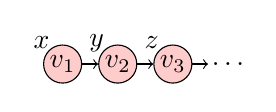
\begin{tikzpicture}[baseline,node distance=7mm, yshift=2pt, every
    node/.style={fill=red!20,circle,draw,inner sep=1pt}]
  \node (x) {$v_1$};
  \node[right of=x] (y) {$v_2$};
  \node[right of=y] (z) {$v_3$};
  \node[right of=z,draw=none,fill=none] (dots) {$\ldots$};
  \node[above left of=x,node distance=3.8mm,draw=none,fill=none] {$x$};
  \node[above left of=y,node distance=3.8mm,draw=none,fill=none] {$y$};
  \node[above left of=z,node distance=3.8mm,draw=none,fill=none] {$z$};
  \path[->] (x) edge (y);
  \path[->] (y) edge (z);
  \path[->] (z) edge (dots);
\end{tikzpicture}
* \displaystyle{\iterStar_{(x,y)\notin S}
  \iterStar_{v} [\text{U}(x,y,v)]
  * \iterStar_{(x,y)\in S}
  \exsts{w}\iterStar_{v\neq w} [\text{U}(x,y,v)]}}
{I_x \cup I_y\cup I_z\cup \cdots}{s}
\]
%
%{\centering \includegraphics[scale=0.232]{Sections/Examples/Images/capSet.pdf}\\}
%
%
The set is represented as a sorted singly-linked list with no
duplicate elements. The list starts at address $x$ with value $v_1$,
points to the next element at address $y$ with value $v_2$, and so
forth. Hereafter, we write $\node{x}{v}{y}$ to denote a node at
address $x$, with value $v$ and successor $y$. 

All nodes of the list reside in a single shared region labelled $s$ and the interference on the list is the combined interference associated with each constituent node. 
Each node at a given address $x$ is associated with a set of update capabilities of the form $[\text{U}(x, y, v)]$ for \emph{all} possible addresses $y$ and \emph{all} possible values $v$. This is to capture all potential successor addresses $y$ and all potential values $v$ that may be stored at address $x$. 
%For instance, since the value $v_{1}$ may be contained in the list at address $x$ before address $y$, there must exist an update capability $[\text{U}(x, y, v_1)]$ to accommodate possible modifications of value $v_{1}$ with respect to $x$ and $y$. 
In order to modify a node, a thread can acquire the lock associated with the node and subsequently claim the relevant update capability.
% 

Since in CAP the capabilities associated with a region can only be generated upon its creation, the shared region is required to keep track of all possible update capabilities $[\text{U}(x, y, v)]$ associated with all addresses $x$ (including those not currently in the domain of the list), all addresses $y$ and all values $v$. At any one point, given $\node{x}{v}{y}$, the only update capability that can be claimed by a thread (through locking) is the one that reflects its current status, namely $[\text{U}(x, y, v)]$. As a result, an auxiliary mathematical set $S$ is used to track those nodes of the list that are currently locked and thus infer which $[\text{U}]$ capabilities have been claimed. The distribution of update capabilities is captured by the two assertions written as the \emph{infinite multiplicative star operator} $\iterStar$. The first part of the assertion states that given any node at address $x$ with successor $y$, if it is not locked, i.e.\ $(x, y) \not\in S$, then {all} of its update capabilities of the form $[\text{U}(x, y, v)]$ lie in the shared region for {all} values $v$. Dually, if it is locked, i.e.\ $(x, y) \in S$, then the update capabilities for {all} values $v$ {but one} ($w \not= v$) are in the shared region.

This CAP set predicate is unnecessarily complicated. It is counter-intuitive
to have to  account for the capabilities associated with   addresses not in the domain of the list. Moreover, each thread observes all nodes in the list and thus needs to account for their associated interference. 

TaDA~\cite{tada} took the first steps towards addressing the above
shortcomings of the CAP approach. TaDA regions are parametric in the
separation algebra of capabilities (called guards).
As such, one can choose a
more suitable algebra to axiomatise the desired behaviour of capabilities. 
%It can  therefore
%provide  a set region which just
%describes the elements of a set. This region  can grow and decrease using
%capabilities and axioms on regions. 
%For instance, when creating the set region $r$, one can choose a capability algebra that satisfies the following axiom.\vspace{-7pt}
%%
%\begin{align*}
%	[\textsc{S}(vs)]_r <=> [\textsc{S}(vs\uplus\{v\})]_r * [\textsc{U}(v)]_r   \\[-20pt]
%\end{align*}
%%
%This axiom effectively ensures that when the set region $r$ contains values $vs$, it may be extended with value $v$, and in doing so claim the the accompanying update capability $[\text{U}(v)]_r$. 
While TaDA's approach is much cleaner than that of CAP, it nevertheless requires the foresight of specifying all desired interference associated with the region upon its creation. 
As such, interference specifications are \emph{static} and cannot be extended with new behaviour even when the existing resources are left untouched. 
On the other hand, as well as being parametric in its capability
separation algebra, the dynamic subjective views of \colosl provide
local reasoning about  the shared resource and its interference. 
%

We proceed with the \colosl proof of the set implementation. Recall from \S\ref{sec:colosl} that \colosl is parametric in the separation algebra of capabilities. We thus instantiate it with a heap-like capability separation algebra that is \emph{stateful} and demonstrate that this allows for a more concise proof.  

We specify the set predicate as the $*$-composition of  subjective
views associated  each node in the singly-linked list as illustrated
by:

{\centering
\begin{tikzpicture}
  \node[inner sep=0pt,outer sep=0pt] (xNy) {$[\nextC{x}{y}] *\null$};
  \node[right of=xNy,circle,draw,fill=blue!15,inner sep=1pt,xshift=2pt] (v1) {$v_1$};
  \node[above left of=v1,node distance=3.8mm,draw=none,fill=none,inner sep=0pt,outer sep=1pt] (x) {$x$};
  \node[fit=(xNy) (v1) (x),rounded corners,rectangle,draw,inner sep=1pt] (n1) {};
  \node[right of=n1, anchor=north west,xshift=0ex] {$I_x$};

  \node[right of=n1,xshift=2.5ex] {$*$};

  \node[inner sep=0pt,outer sep=0pt,right of=xNy,node distance=2.7cm] (yNz) {$[\nextC{y}{z}] *\null$};
  \node[right of=yNz,circle,draw,fill=blue!15,inner sep=1pt,xshift=2pt] (v2) {$v_2$};
  \node[above left of=v2,node distance=3.8mm,draw=none,fill=none,inner sep=0pt,outer sep=0pt] (y) {$y$};
  \node[fit=(yNz) (v2) (y),rounded corners,rectangle,draw,inner sep=1pt] (n2) {};
  \node[right of=n2, anchor=north west,xshift=0ex] {$I_y$};
  \node[right of=n2,xshift=2.5ex] {$*$};

  \node[inner sep=0pt,outer sep=0pt,right of=yNz,node distance=2.9cm] (zN) {$[\nextC{z}{\dots}] *\null$};
  \node[right of=zN,circle,draw,fill=blue!15,inner sep=1pt,xshift=5pt] (v3) {$v_3$};
  \node[above left of=v3,node distance=3.8mm,draw=none,fill=none,inner sep=0pt,outer sep=1pt] (z) {$z$};
  \node[fit=(zN) (v3) (z),rounded corners,rectangle,draw,inner sep=1pt] (n3) {};
  \node[right of=n3, anchor=north west,xshift=1ex] {$I_z$};
  \node[right of=n3,xshift=3.5ex] {$*$};

  \node[inner sep=0pt,outer sep=0pt,right of=zN,node distance=2.3cm] (dots) {$\cdots$};

  \path[->] (v1.north east) edge[semithick,bend left=55] (n2.west);
  \path[->] (v2.north east) edge[semithick,bend left=55] (n3.west);
  \path[->] (v3.north east) edge[semithick,bend left=55] (dots.north west);
\end{tikzpicture}\\}
\noindent  The interference on each subjective view is limited to the
node in question. Associated with each node at address $x$ is a
``next'' capability $[\nextC{x}{y}]$ that tracks its successor
$y$. This is analogous to the $[\text{U}(x, y, v)]$ capability of CAP
and we shortly demonstrate how it is utilised in our reasoning. 

Since \colosl allows for {dynamic} extension of the shared state, we do not need to account for capabilities associated with all addresses. Instead, fresh capabilities are generated dynamically as needed. We demonstrate this by giving a reasoning outline of the \li{add(}$v'$\li{)} method that adds value $v'$ to the set by inserting it in the sorted list.
Suppose $v_2 < v' < v_3$, and thus a new node $w$ with value $v'$ is
to be inserted after node $y$.  The operating thread proceeds by
traversing the list by hand-over-hand locking until it reaches node
$y$. It then locks $y$ and claims its next pointer and moves it to its
local state, as allowed by $I_y$. Subsequently, the shared state is
{extended} by the resources associated with the new node and its
associated capabilities ($[\nextC{w}{z}]$) are generated on the fly as
illustrated by:\vspace{0pt}

{\centering
\begin{tikzpicture}
  \node[inner sep=0pt,outer sep=0pt] (xNy) {$[\nextC{x}{y}] *\null$};
  \node[right of=xNy,circle,draw,fill=blue!15,inner sep=1pt,xshift=2pt] (v1) {$v_1$};
  \node[above left of=v1,node distance=3.8mm,draw=none,fill=none,inner sep=0pt,outer sep=1pt] (x) {$x$};
  \node[fit=(xNy) (v1) (x),rounded corners,rectangle,draw,inner sep=1pt] (n1) {};
  \node[right of=n1, anchor=north west,xshift=0ex] {$I_x$};

  \node[right of=xNy,node distance=1.7cm] {$*$};

  \node[inner sep=0pt,outer sep=0pt,right of=xNy,node distance=2.7cm] (yNz) {$[\nextC{y}{z}] *\null$};
  \node[right of=yNz,circle,draw,fill=blue!15,inner sep=1pt,xshift=2pt] (v2) {$v_2$};
  \node[above left of=v2,node distance=3.8mm,draw=none,fill=none,inner sep=0pt,outer sep=0pt] (y) {$y$};
  \node[fit=(yNz) (v2) (y),rounded corners,rectangle,draw,inner sep=1pt] (n2) {};
  \node[right of=n2, anchor=north west,xshift=0ex] {$I_y$};
  \node[right of=yNz,node distance=1.7cm] {$*$};

  \node[inner sep=0pt,outer sep=0pt,right of=yNz,node distance=2.7cm] (wNz) {$[\nextC{w}{{\color{red}z}}] *\null$};
  \node[right of=wNz,circle,draw,fill=blue!15,inner sep=1pt,xshift=2pt] (v4) {$v'$};
  \node[above left of=v4,node distance=3.8mm,draw=none,fill=none,inner sep=0pt,outer sep=1pt] (w) {$w$};
  \node[fit=(wNz) (v4) (w),rounded corners,rectangle,draw,inner sep=1pt] (n4) {};
  \node[right of=n4, anchor=north west,xshift=0.4ex] {$I_w$};
  \node[right of=wNz,node distance=1.75cm] {$*$};

  \node[inner sep=0pt,outer sep=0pt,right of=wNz,node distance=2.9cm] (zN) {$[\nextC{z}{\dots}] *\null$};
  \node[right of=zN,circle,draw,fill=blue!15,inner sep=1pt,xshift=5pt] (v3) {$v_3$};
  \node[above left of=v3,node distance=3.8mm,draw=none,fill=none,inner sep=0pt,outer sep=1pt] (z) {$z$};
  \node[fit=(zN) (v3) (z),rounded corners,rectangle,draw,inner sep=1pt] (n5) {};
  \node[right of=n5, anchor=north west,xshift=1ex] {$I_z$};
  \node[right of=zN,node distance=1.8cm] {$*$};

  \node[inner sep=0pt,outer sep=0pt,right of=zN,node distance=2.3cm] (dots) {$\cdots$};

  \draw[fill=red,semithick] (v2.north east) + (-2pt,-2pt)  rectangle +(2pt,2pt);
  \draw[semithick] (v2.north east) + (2pt,2pt) arc (0:180:2pt);  
  \path[->] (v1.north east) edge[semithick,bend left=55] (n2.west);
  \path[->] (v3.north east) edge[semithick,bend left=55] (dots.north west);
  \path[->] (v4.north east) edge[semithick,bend left=55,red] (n5.west);
\end{tikzpicture}\\}
%
%{\centering \includegraphics[scale=0.25]{Sections/Examples/Images/add1.pdf}\\}
%
%At this point, since the locking thread holds the next pointer of $y$ in its local state, it modifies it to point to the new node $w$. It then unlocks $y$ and returns its next pointer to the shared state. However, the interference assertion associated with node $y$ ($I_y$) allows the node to be unlocked in three possible ways. Either its successor has not changed from its old value $z$ (tracked by $\nextC{y}{z}$); \emph{or} it has been redirected to $z$'s successor (when $z$ is being deleted); \emph{or} it has been directed to a new node whose successor is $z$ (a new node is inserted between $y$ and $z$). When adding a new node after $y$, the latter of the possibilities is applicable and thus the unlocking thread must demonstrate that the new node ($w$) does indeed point to $z$. In order to establish this condition, we use the (\mergeRule) principle in our reasoning to combine the subjective views of $y$ and $w$ as follows.
\noindent Since the locking thread holds the next pointer of $y$ in
its local state, it modifies it to point to the new node $w$. It then
unlocks $y$ and returns its next pointer to the shared state. When
inserting a new node between $y$ and $z$, the associated interference
assertion $I_y$ allows $y$ to be unlocked only if it has been directed
to a new node whose successor is $z$. As such, the unlocking thread
must demonstrate that the new node $w$ does indeed point to $z$. In
order to establish this, we use the \mergeRule principle to combine
the subjective views of $y$ and $w$ as follows: \vspace{0pt}

{\centering
\begin{tikzpicture}
  \node[inner sep=0pt,outer sep=0pt] (xNy) {$[\nextC{x}{y}] *\null$};
  \node[right of=xNy,circle,draw,fill=blue!15,inner sep=1pt,xshift=2pt] (v1) {$v_1$};
  \node[above left of=v1,node distance=3.8mm,draw=none,fill=none,inner sep=0pt,outer sep=1pt] (x) {$x$};
  \node[fit=(xNy) (v1) (x),rounded corners,rectangle,draw,inner sep=1pt] (n1) {};
  \node[right of=n1, anchor=north west,xshift=0ex] {$I_x$};

  \node[right of=xNy,node distance=1.7cm] {$*$};

  \node[inner sep=0pt,outer sep=0pt,right of=xNy,node distance=2.7cm] (yNz) {$[\nextC{y}{z}] *\null$};
  \node[right of=yNz,circle,draw,fill=blue!15,inner sep=1pt,xshift=2pt] (v2) {$v_2$};
  \node[above left of=v2,node distance=3.8mm,draw=none,fill=none,inner sep=0pt,outer sep=0pt] (y) {$y$};

  \node[inner sep=0pt,outer sep=0pt,right of=v2,node distance=1.25cm] (wNz) {$\null*[\nextC{w}{z}] *\null$};
  \node[right of=wNz,circle,draw,fill=blue!15,inner sep=1pt,xshift=7pt] (v4) {$v'$};
  \node[above left of=v4,node distance=3.8mm,draw=none,fill=none,inner sep=0pt,outer sep=1pt] (w) {$w$};
  \node[fit=(wNz) (v4) (w) (yNz) (v2) (y),rounded corners,rectangle,draw,inner sep=1pt] (n4) {};
  \node[right of=n4, anchor=north west,xshift=8.4ex] {$I_y\cup I_w$};
  \node[right of=wNz,node distance=2.6cm] {$*$};

  \node[inner sep=0pt,outer sep=0pt,right of=wNz,node distance=3.8cm] (zN) {$[\nextC{z}{\dots}] *\null$};
  \node[right of=zN,circle,draw,fill=blue!15,inner sep=1pt,xshift=5pt] (v3) {$v_3$};
  \node[above left of=v3,node distance=3.8mm,draw=none,fill=none,inner sep=0pt,outer sep=1pt] (z) {$z$};
  \node[fit=(zN) (v3) (z),rounded corners,rectangle,draw,inner sep=1pt] (n5) {};
  \node[right of=n5, anchor=north west,xshift=1ex] {$I_z$};
  \node[right of=zN,node distance=1.8cm] {$*$};

  \node[inner sep=0pt,outer sep=0pt,right of=zN,node distance=2.3cm] (dots) {$\cdots$};

  \draw[fill=red,semithick] (v2.north east) + (-2pt,-2pt)  rectangle +(2pt,2pt);
  \draw[semithick] (v2.north east) + (2pt,2pt) arc (0:180:2pt);  
  \path[->] (v1.north east) edge[semithick,bend left=55] (n2.west);
  \path[->] (v3.north east) edge[semithick,bend left=55] (dots.north west);
  \path[->] (v4.north east) edge[semithick,bend left=55] (n5.west);
\end{tikzpicture}\\}
%
%x{\centering \includegraphics[scale=0.25]{Sections/Examples/Images/add2.pdf}\\}
%
%Finally, node $y$ is unlocked; its updated next pointer is returned to the shared state and its next capability is modified accordingly to reflect its new successor. Using the (\copyRule), (\forgetRule) and (\shiftRule) principles \textit{ad seriatim}, we can once again obtain the set predicate with the new node $w$ inserted. 
\noindent Finally, $y$ is unlocked; its next pointer is returned to the shared state and its next capability is modified to reflect its new successor. Using the \copyRule, \forgetRule and \shiftRule principles in order, we obtain the set predicate with $w$ inserted. \vspace{0pt}

{\centering
\begin{tikzpicture}
  \node[inner sep=0pt,outer sep=0pt] (xNy) {$[\nextC{x}{y}] *\null$};
  \node[right of=xNy,circle,draw,fill=blue!15,inner sep=1pt,xshift=2pt] (v1) {$v_1$};
  \node[above left of=v1,node distance=3.8mm,draw=none,fill=none,inner sep=0pt,outer sep=1pt] (x) {$x$};
  \node[fit=(xNy) (v1) (x),rounded corners,rectangle,draw,inner sep=1pt] (n1) {};
  \node[right of=n1, anchor=north west,xshift=0ex] {$I_x$};

  \node[right of=xNy,node distance=1.7cm] {$*$};

  \node[inner sep=0pt,outer sep=0pt,right of=xNy,node distance=2.7cm] (yNz) {$[\nextC{y}{{\color{red}w}}] *\null$};
  \node[right of=yNz,circle,draw,fill=blue!15,inner sep=1pt,xshift=2pt] (v2) {$v_2$};
  \node[above left of=v2,node distance=3.8mm,draw=none,fill=none,inner sep=0pt,outer sep=0pt] (y) {$y$};
  \node[fit=(yNz) (v2) (y),rounded corners,rectangle,draw,inner sep=1pt] (n2) {};
  \node[right of=n2, anchor=north west,xshift=0ex] {$I_y$};
  \node[right of=yNz,node distance=1.7cm] {$*$};

  \node[inner sep=0pt,outer sep=0pt,right of=yNz,node distance=2.7cm] (wNz) {$[\nextC{w}{z}] *\null$};
  \node[right of=wNz,circle,draw,fill=blue!15,inner sep=1pt,xshift=2pt] (v4) {$v'$};
  \node[above left of=v4,node distance=3.8mm,draw=none,fill=none,inner sep=0pt,outer sep=1pt] (w) {$w$};
  \node[fit=(wNz) (v4) (w),rounded corners,rectangle,draw,inner sep=1pt] (n4) {};
  \node[right of=n4, anchor=north west,xshift=0.4ex] {$I_w$};
  \node[right of=wNz,node distance=1.75cm] {$*$};

  \node[inner sep=0pt,outer sep=0pt,right of=wNz,node distance=2.9cm] (zN) {$[\nextC{z}{\dots}] *\null$};
  \node[right of=zN,circle,draw,fill=blue!15,inner sep=1pt,xshift=5pt] (v3) {$v_3$};
  \node[above left of=v3,node distance=3.8mm,draw=none,fill=none,inner sep=0pt,outer sep=1pt] (z) {$z$};
  \node[fit=(zN) (v3) (z),rounded corners,rectangle,draw,inner sep=1pt] (n5) {};
  \node[right of=n5, anchor=north west,xshift=1ex] {$I_z$};
  \node[right of=zN,node distance=1.8cm] {$*$};

  \node[inner sep=0pt,outer sep=0pt,right of=zN,node distance=2.3cm] (dots) {$\cdots$};

  \path[->] (v1.north east) edge[semithick,bend left=55] (n2.west);
  \path[->] (v2.north east) edge[semithick,bend left=55,red] (n4.west);
  \path[->] (v3.north east) edge[semithick,bend left=55] (dots.north west);
  \path[->] (v4.north east) edge[semithick,bend left=55] (n5.west);
\end{tikzpicture}\\}
%
%{\centering \includegraphics[scale=0.25]{Sections/Examples/Images/add3.pdf}\\}
%
We can reason about the \li{remove} operation in a similar
fashion. The dynamic extension afforded by the \extendRule\ principle
allows us to generate new capabilities only when needed and thus gives
way to a concise proof. 
%
Moreover, rather than having a distinct capability to modify the element at address $x$, for each possible successor address $y$ (as with $[\text{U}(x, y, v)]$ in CAP), we appeal to a single capability of the form $[\nextC{x}{y}]$ that is modified to $[\nextC{x}{y'}]$ whenever $x$'s successor changes from $y$ to $y'$.
%the capability is modified accordingly to record the changes to the successor address. 
%
Lastly, using the reasoning principles of \mergeRule, \forgetRule,
\shiftRule\ and \copyRule, we can grow and shrink our subjective views
as needed. This means that,  at any one point, we only view the relevant parts of the shared state. 
%
The technical details can be found in~\cite{colosl-tr14}. 

\section{Conclusions}
\label{sec:conclusion}

Well, that was awesome.

Future work: because we are able to specify shared state and
interferences locally, there is hope that \colosl can be adapted to
reason about distributed systems as well, as in our motivating example
of \S\ref{sec:intuition}.

\julescomment{This is a brain dump. Doesn't have to make it in the
  submitted version.}

One of the new paradigms of \colosl is the ability to manipulate the
interference relation, via \emph{shifting}. The focus of this paper
has largely been on manipulations of the spatial components of
subjective views, and the treatment of shifting has been left at the
minimum we needed to cover our range of examples. This opens the way
to more fine-grained reasoning about interferences. For instance, a
process who never receives a capability could safely over-approximate
the corresponding interference. Conversely, a process who never gives
a capability away could safely under-approximate the corresponding
interference relation. In \colosl, this is not yet allowed, as
interferences can only be shifted to equivalent ones, the only
exception being the ability to forget actions that have no visible
effect on the current subjective state. One could imagine tracking
which process is allowed to own which capability to be more flexible
in this instance. (if that can be useful at all?)


% POPL recommends abbrvnat bibliography style.
%% \bibliographystyle{abbrvnat}
\bibliographystyle{plain_better}
\bibliography{biblio}
% The bibliography should be embedded for final submission.


\end{document}
